\chapter{Interpretation}
\label{ch:9}

% **************************** Define Graphics Path **************************
\ifpdf
    \graphicspath{{Chapter9/Figs/Raster/}{Chapter9/Figs/PDF/}{Chapter9/Figs/}}
\else
    \graphicspath{{Chapter9/Figs/Vector/}{Chapter9/Figs/}}
\fi

%********************************** % First Section  *************************************
\section{Signal Acceptance}  %Section - 1.1 
\label{sec:interpretation_acceptance}

Model acceptance is determined as a function of analysis category (\nb, \nj) and
\HT bin. This calculation is performed individually for each mass point in the
scan plane for both the hadronic selection and muon selection (to determine 
signal contamination in the control region). Interpretations are made using a
selected subset of the analysis 
categories, but an inclusive \HT selection. The analysis categories used are 
selected after an inspection of each for their significance given signal 
injection from specific mass points (REF).

\subsection{T2cc}
Signal efficiency times acceptance for the \texttt{T2cc} model is shown in 
figure~\ref{fig:sms-t2cc-sig}. The strongest acceptance is seen in the \njlow, 
\nb=0 analysis category, where efficiencies are around the percent level. At 
small mass splittings, nearest the kinematically inaccessible diagonal region, 
acceptance is due to hard initial state radiation (ISR) jets balancing a soft 
SUSY decay system. Small mass splittings imply little energy is available for 
decay products to gain sufficient momentum to be in acceptance, and therefore 
become invisible to the analysis. In order for such an event to pass the 
selection criteria of the signal sample, hard ISR jets are required to be within
kinematic acceptance and boosting this decay system. Moving away from the 
diagonal to increasing values of \deltam indicates a drop in acceptance, 
eventually leading to an increase due to a competing effect from the increase in
available kinematic phase space. Far from the diagonal, decay products are able 
to gain sufficient momentum to enter acceptance, thereby becoming visible. There
is still a dependence on ISR jets boosting this system, however crucially jets 
originating from charm quarks could now be observed. Due to this, contributions 
to acceptance increase not only for this \nb=0 category, but similarly for \nb=1
categories, due to mistagging probabilities, where no real acceptance is 
observed at small \deltam.

Finally, reasonable acceptance is observed in the \njhigh categories, 
predominantly away from the diagonal. Again, given the increased kinematic phase
space of the larger mass splitting scenarios, more jets can potentially be in 
acceptance.

\emph{somewhere describe the significance plots, leading to the choice of these 
particularly categories.}

Signal contamination in the \mj selection is shown to be negligible, given the 
lack of leptonic activity in the final state.

\emph{what about stop mass?}

% should be v25!
\begin{figure}[ht!]
  \centering
  \begin{subfigure}[b]{0.47\textwidth}
    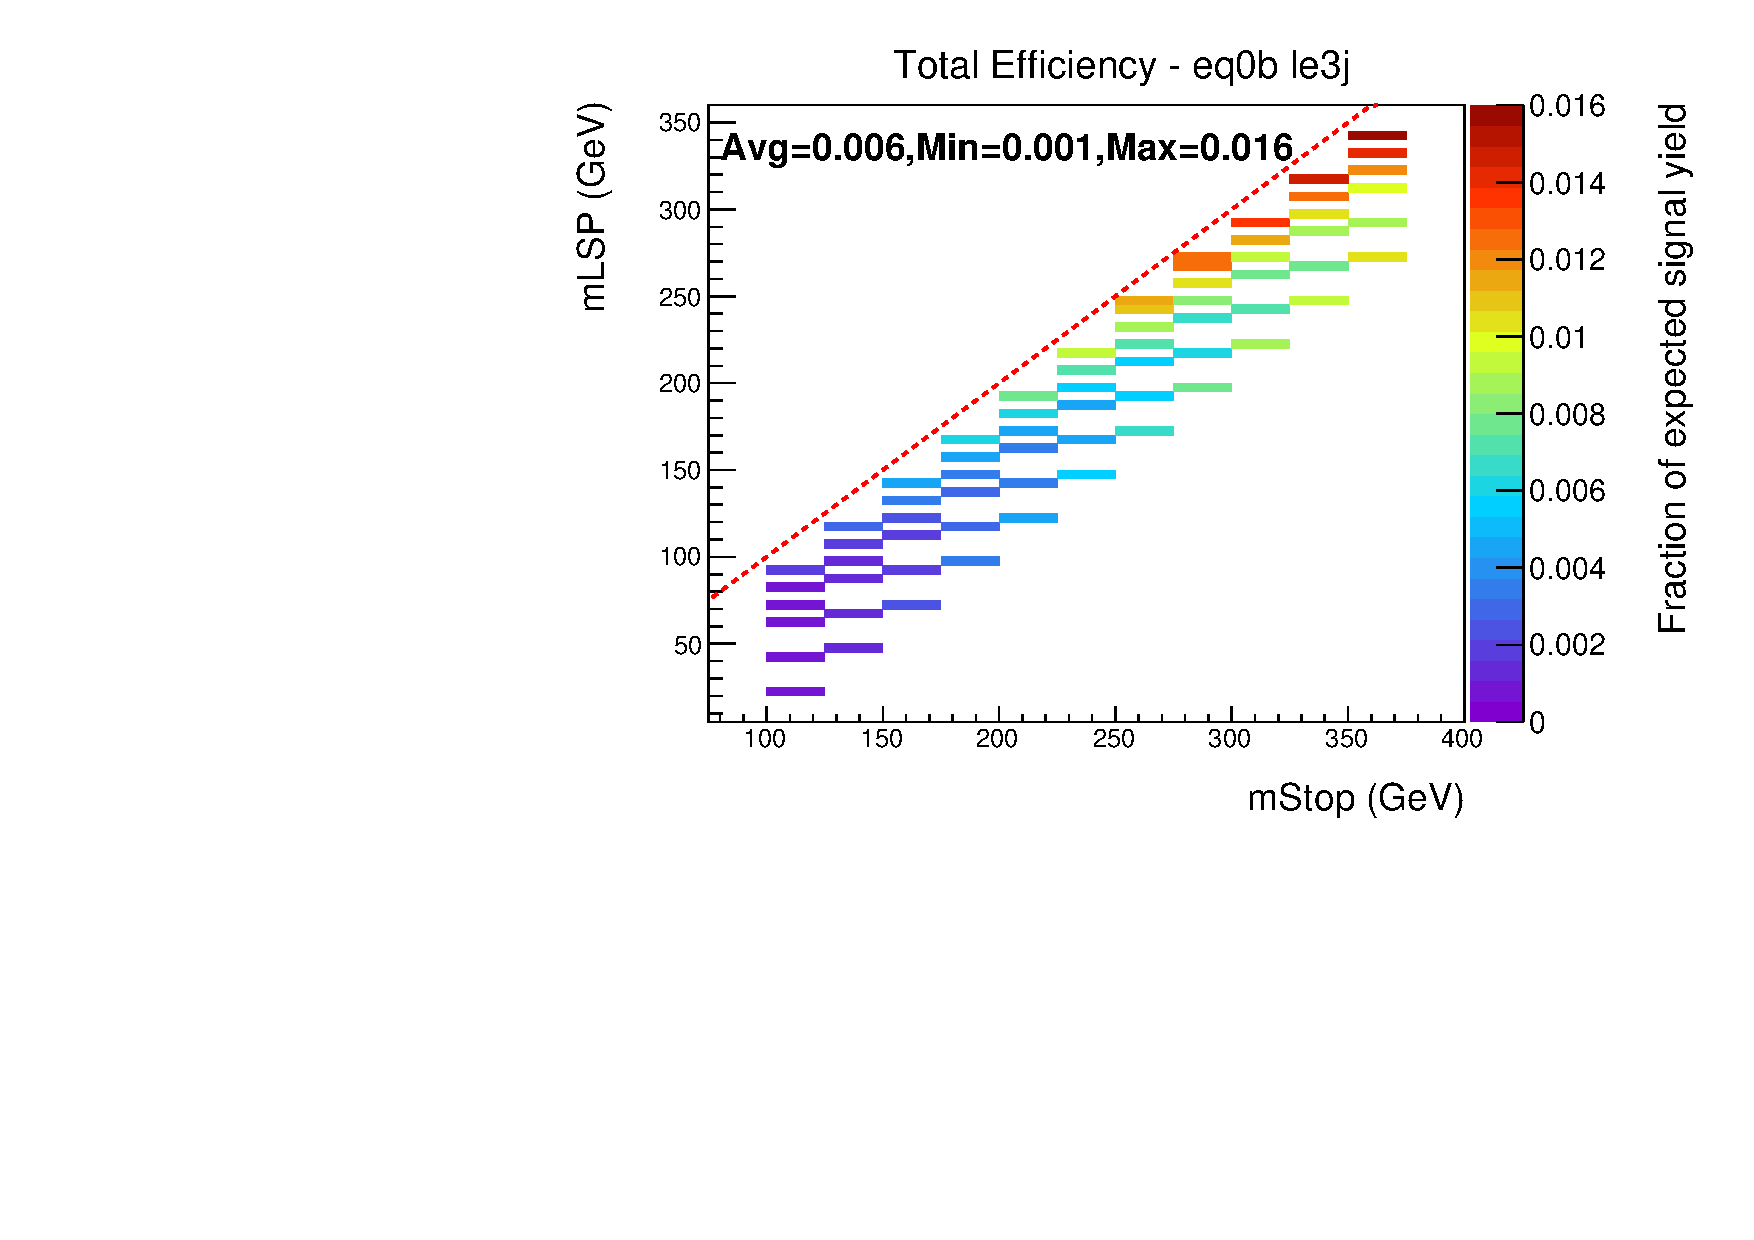
\includegraphics[width=\textwidth]{Figs/sms/t2cc/v24/T2cc_v24_had_eff_maps_eq0b_le3j_SITV.pdf}
    \caption{Signal region, (2--3,0)}
    \label{fig:t2cc_sig_eff_le3j_0b}
  \end{subfigure}
  \begin{subfigure}[b]{0.47\textwidth}
    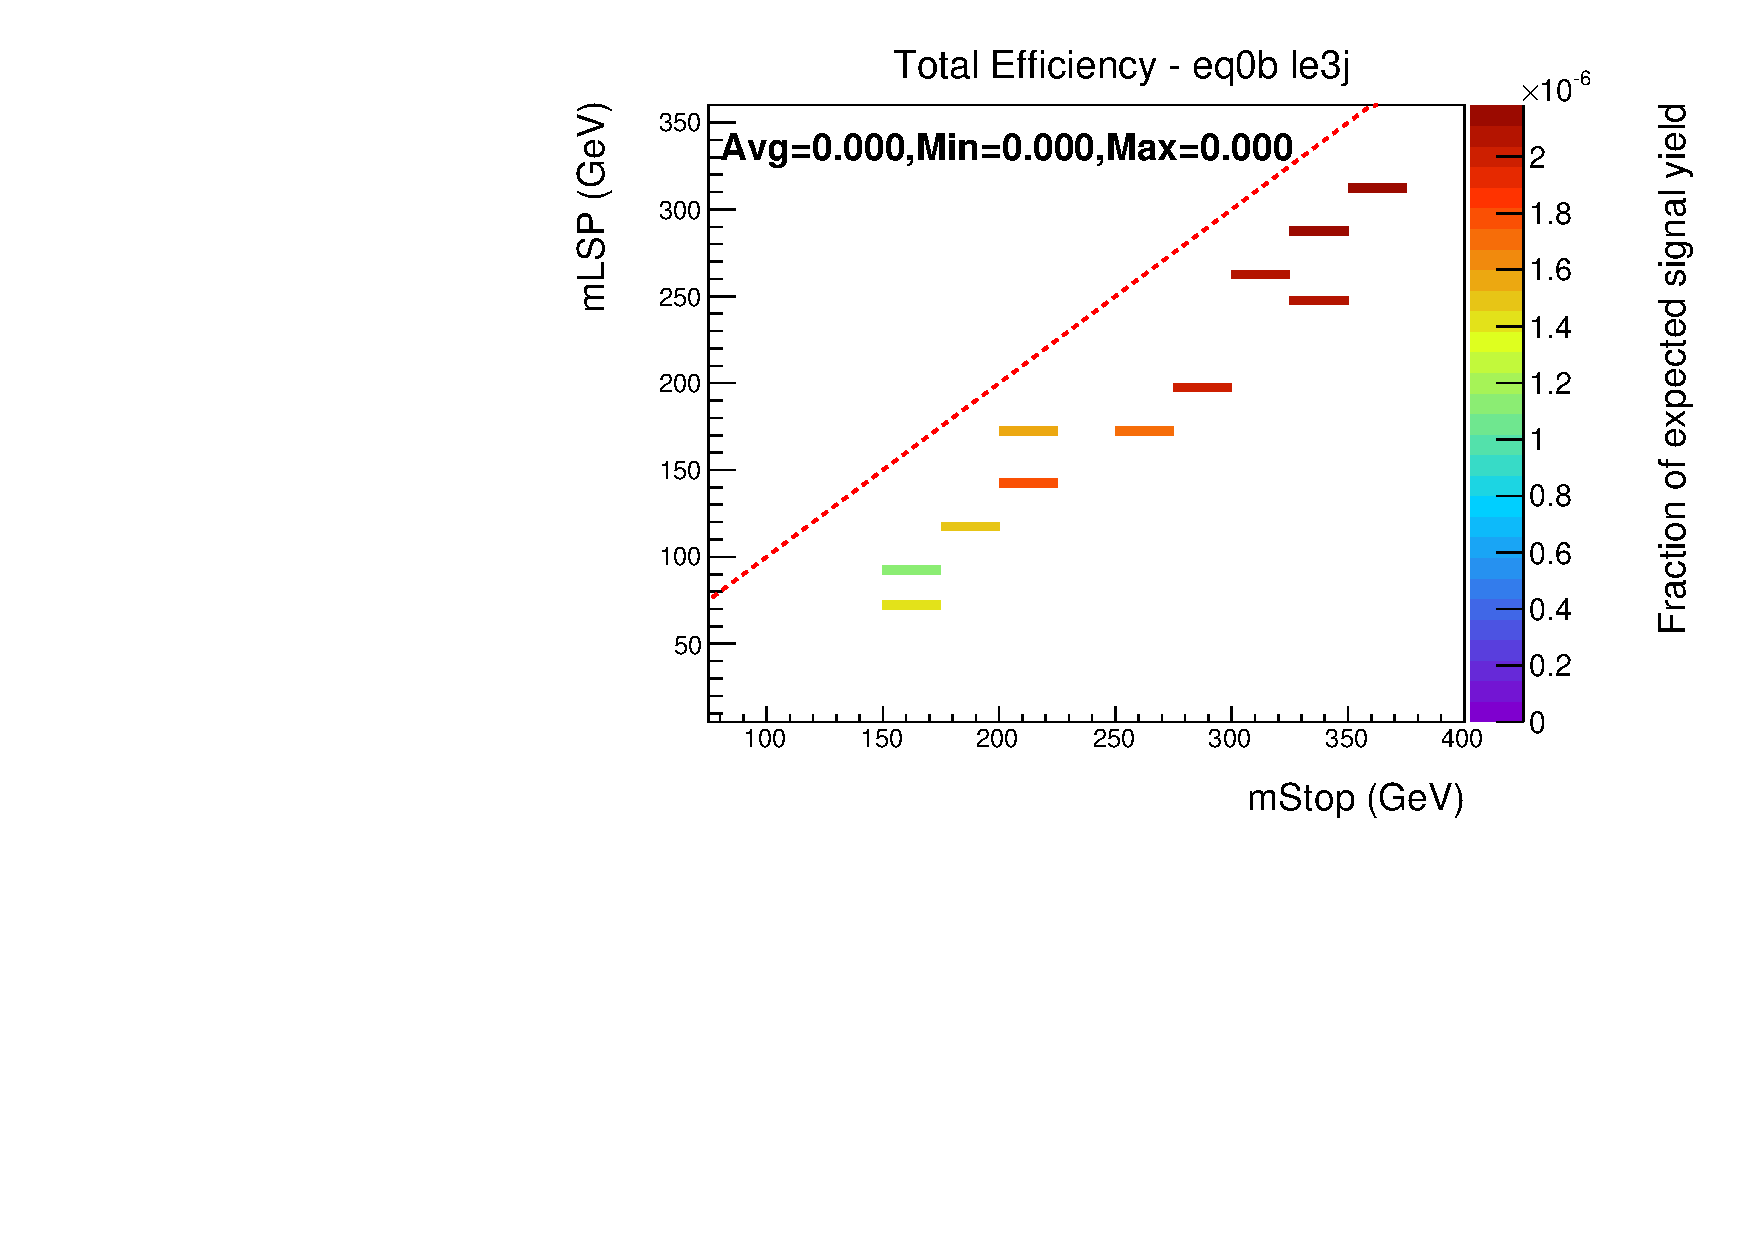
\includegraphics[width=\textwidth]{Figs/sms/t2cc/v24/T2cc_v24_muon_eff_maps_eq0b_le3j_SITV.pdf}
    \caption{\mj region, (2--3,0)}
    \label{fig:t2cc_mu_eff_le3j_0b}
  \end{subfigure} \\
  \begin{subfigure}[b]{0.47\textwidth}
    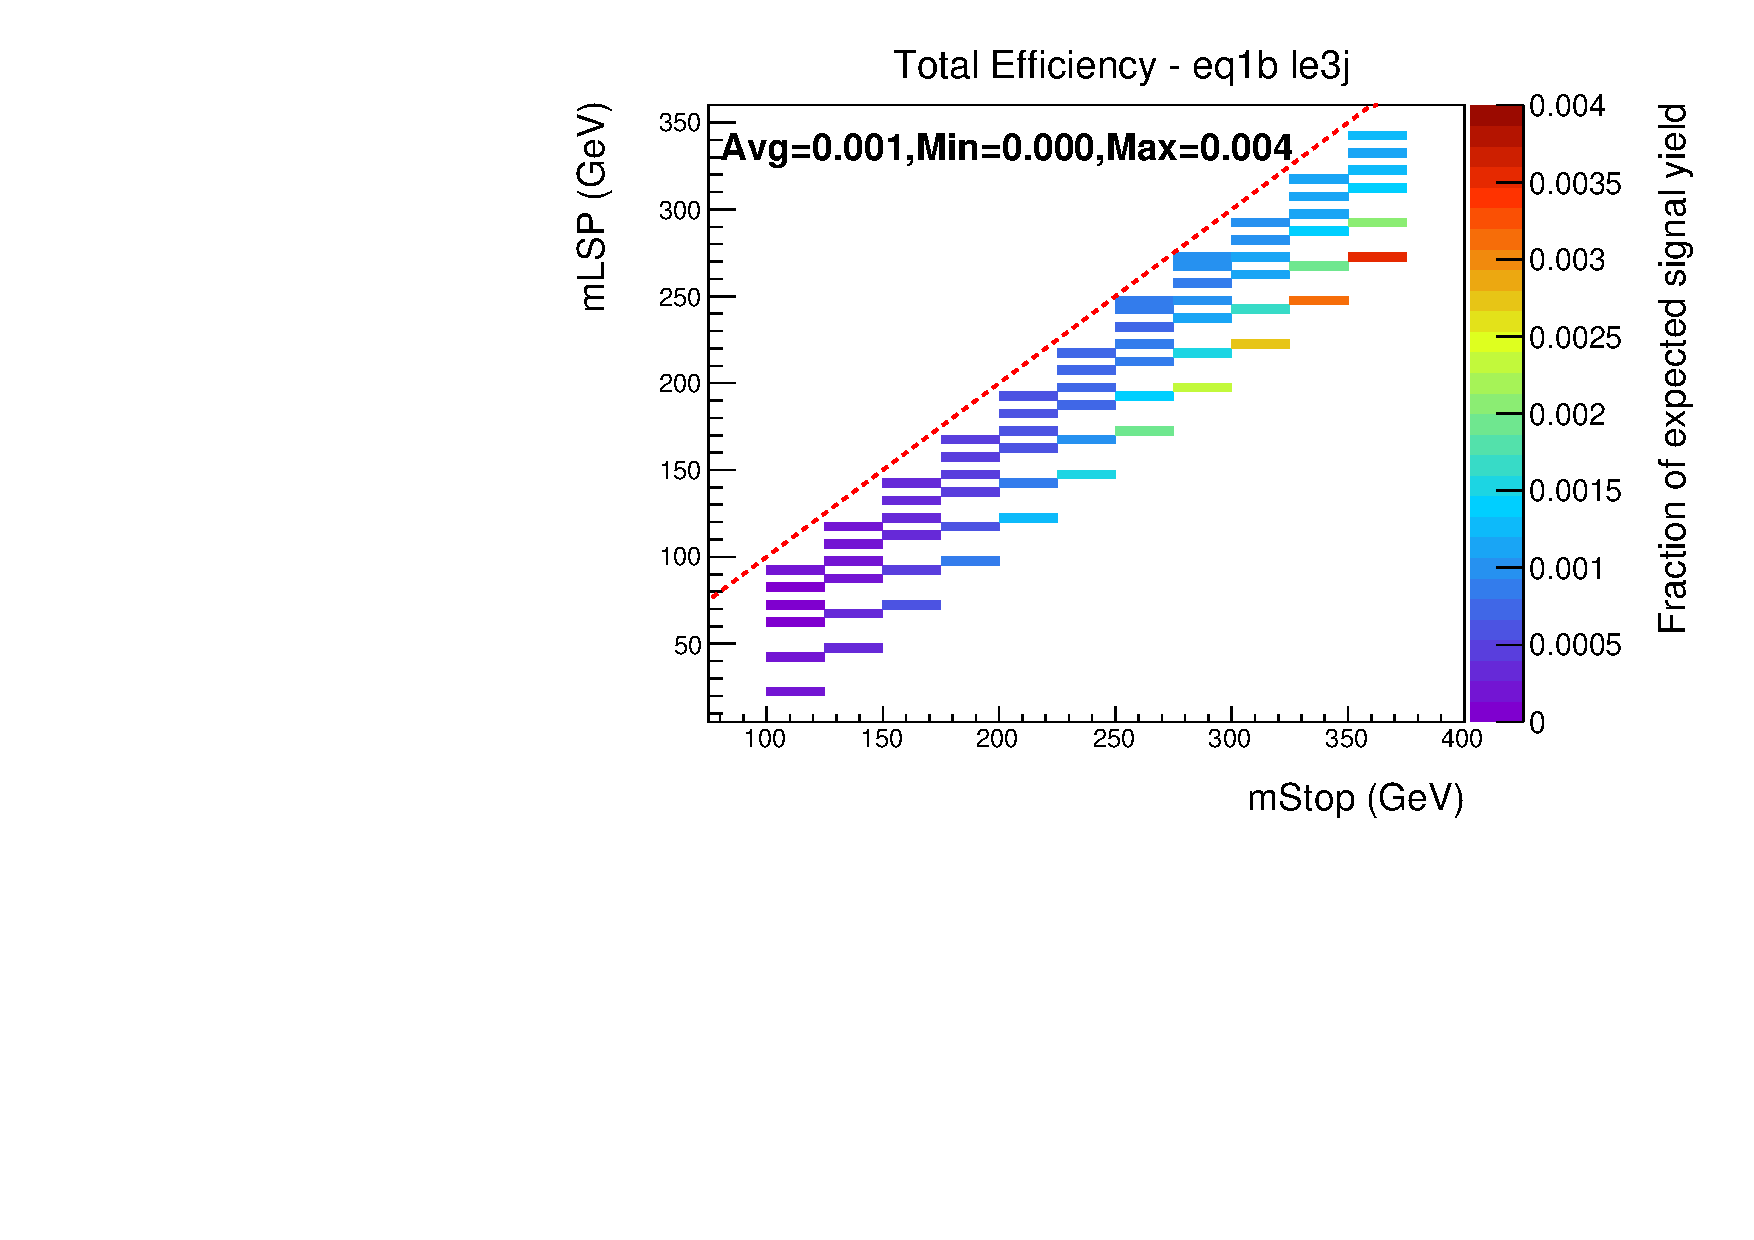
\includegraphics[width=\textwidth]{Figs/sms/t2cc/v24/T2cc_v24_had_eff_maps_eq1b_le3j_SITV.pdf}
    \caption{Signal region, (2--3,1)}
    \label{fig:t2cc_sig_eff_le3j_1b}
  \end{subfigure}
  \begin{subfigure}[b]{0.47\textwidth}
    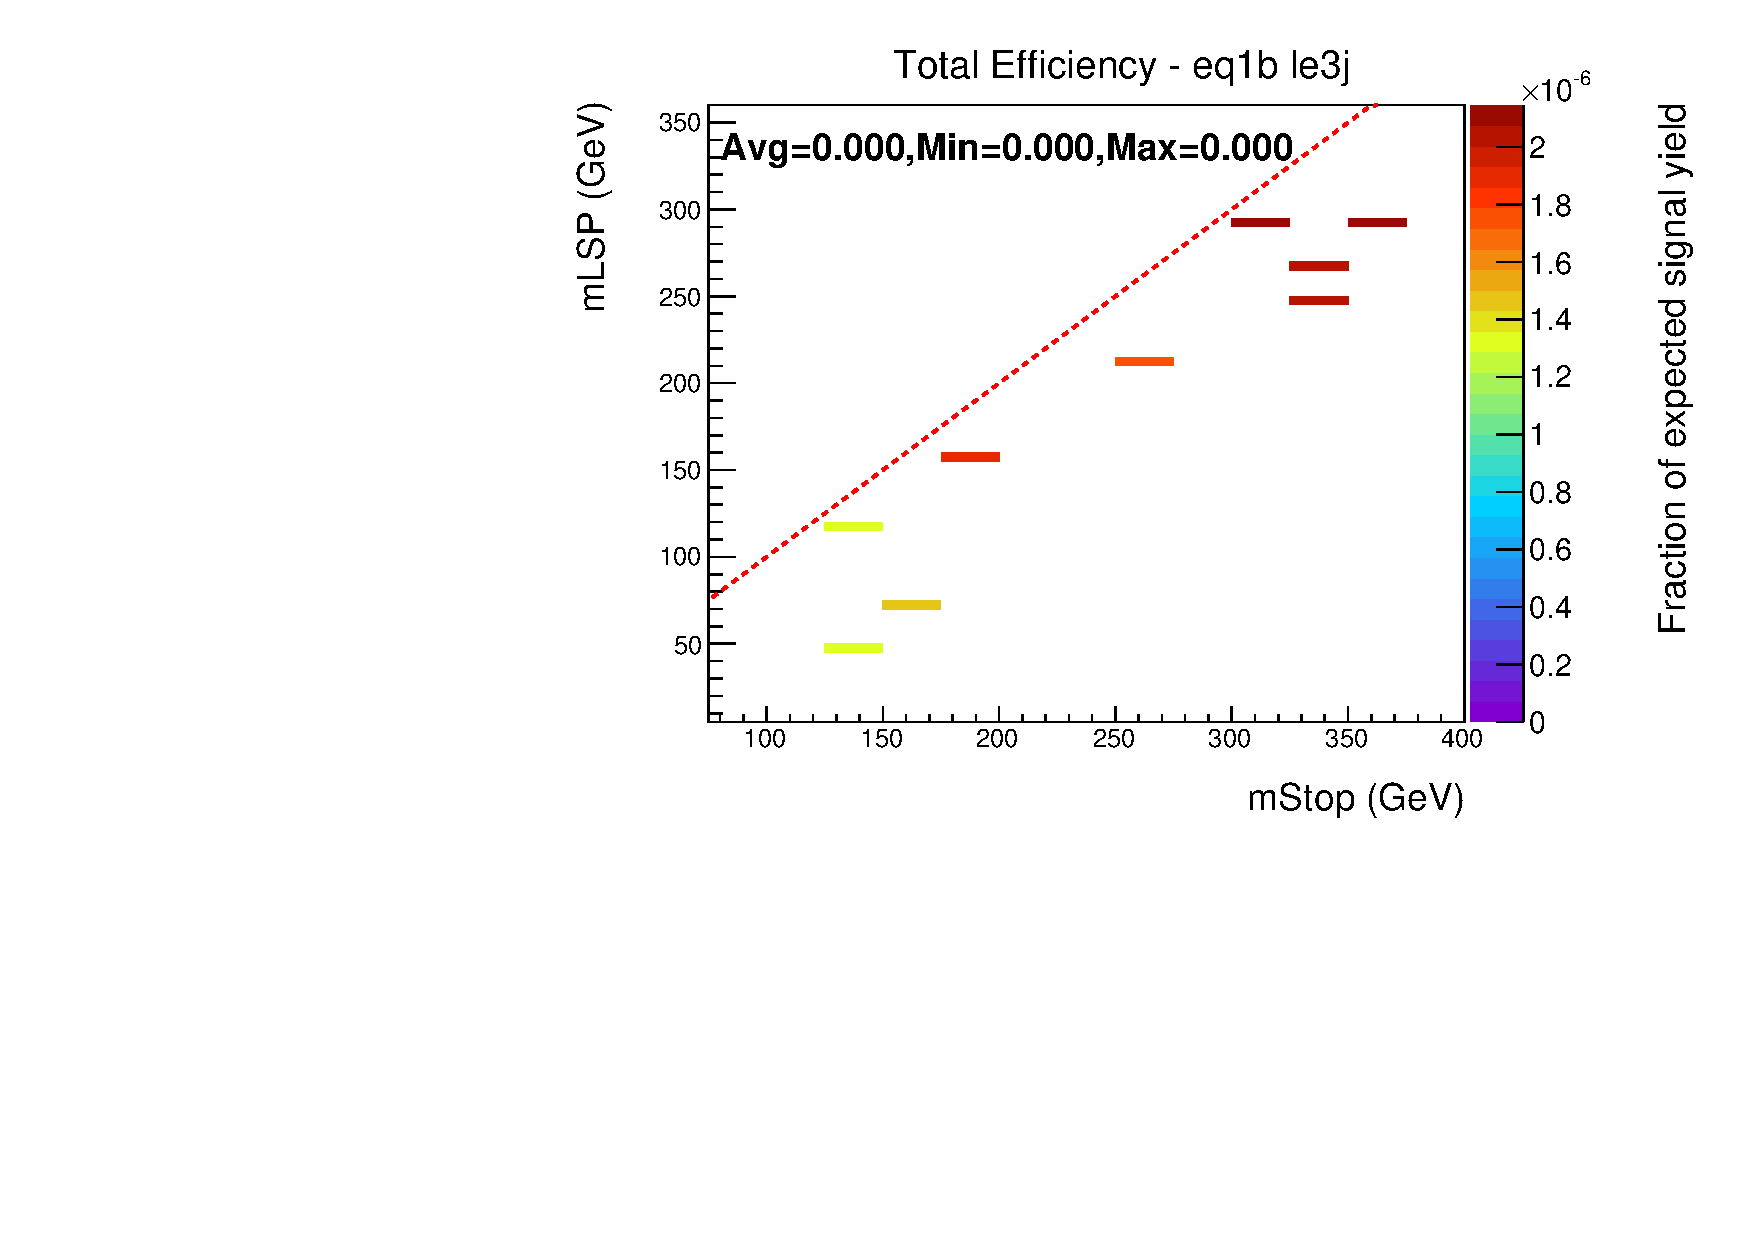
\includegraphics[width=\textwidth]{Figs/sms/t2cc/v24/T2cc_v24_muon_eff_maps_eq1b_le3j_SITV.pdf}
    \caption{\mj region, (2--3,1)}
    \label{fig:t2cc_mu_eff_le3j_1b}
  \end{subfigure} \\
  \begin{subfigure}[b]{0.47\textwidth}
    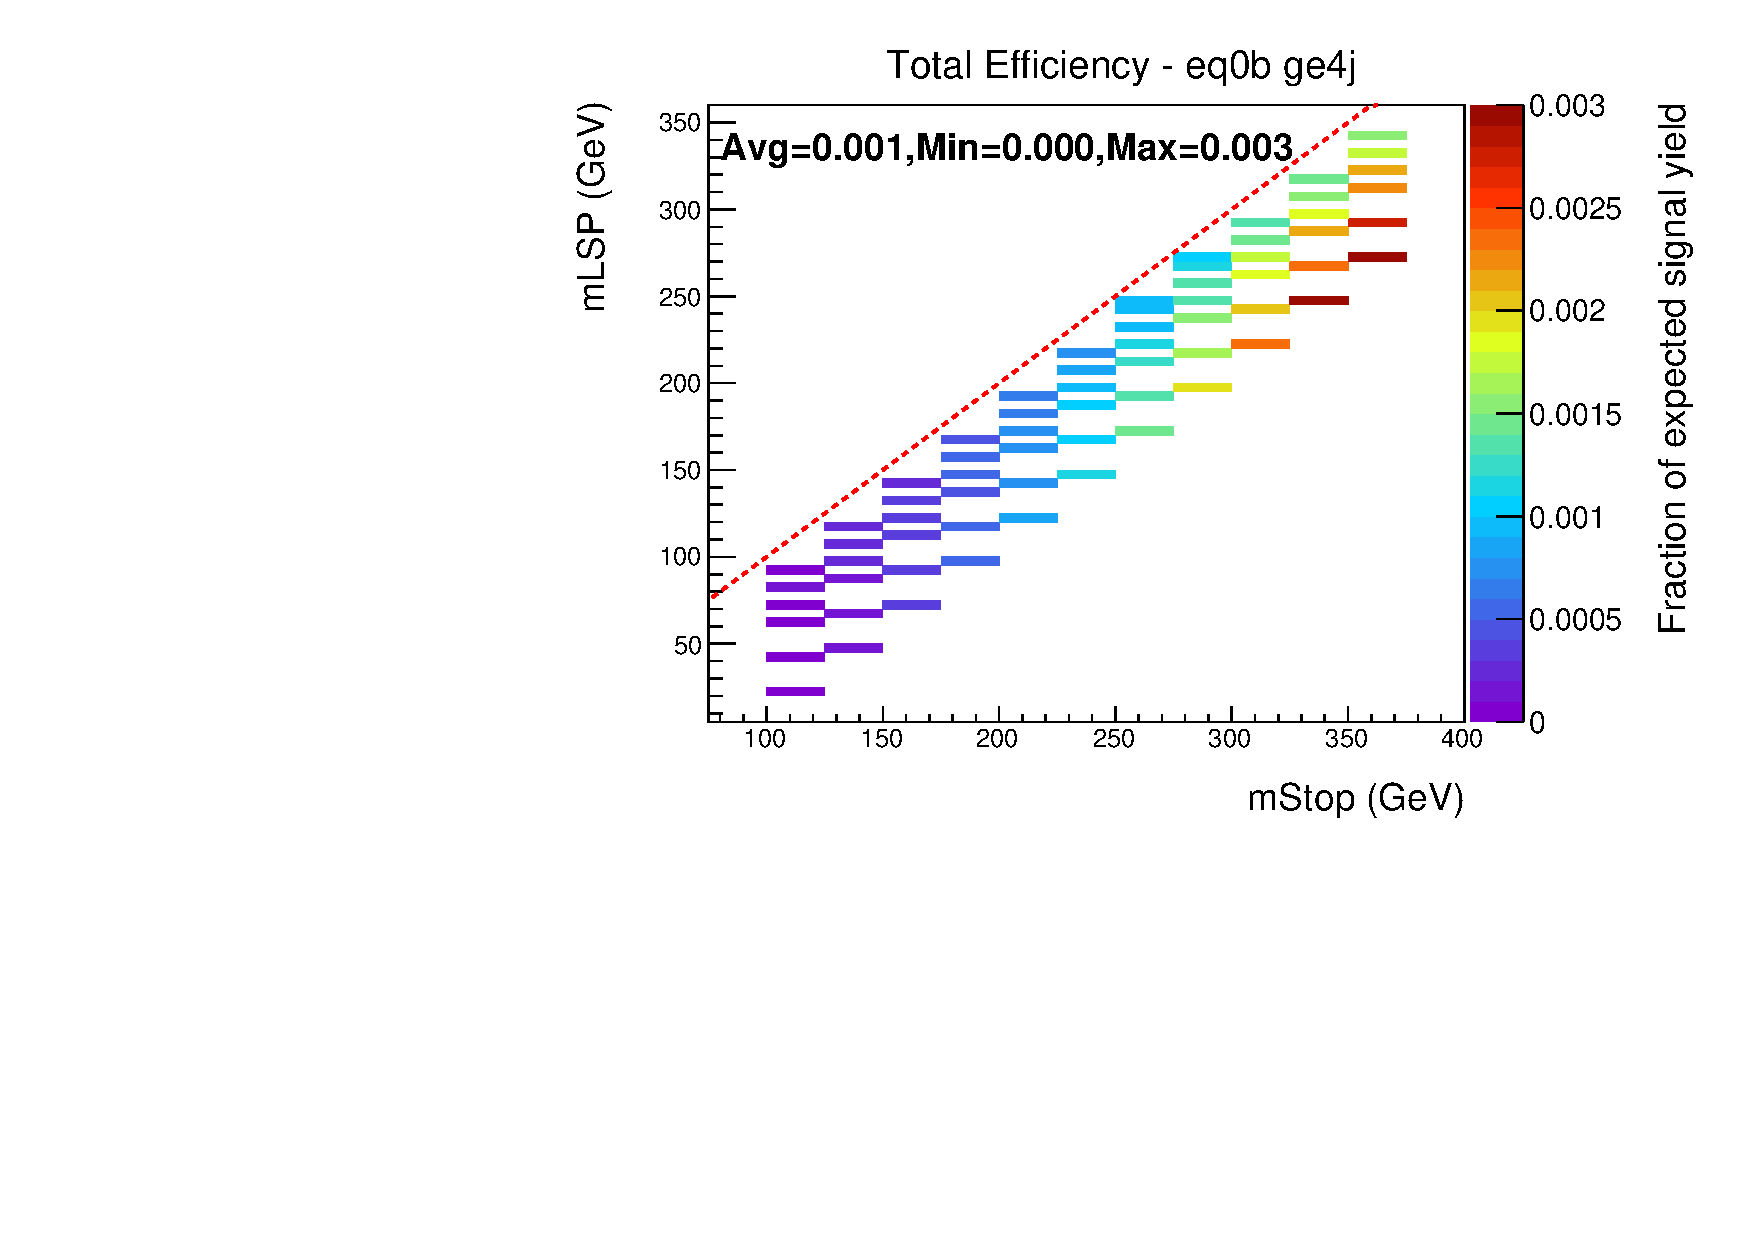
\includegraphics[width=\textwidth]{Figs/sms/t2cc/v24/T2cc_v24_had_eff_maps_eq0b_ge4j_SITV.pdf}
    \caption{Signal region, ($\geq 4$,0)}
    \label{fig:t2cc_sig_eff_ge4j_0b}
  \end{subfigure}
  \begin{subfigure}[b]{0.47\textwidth}
    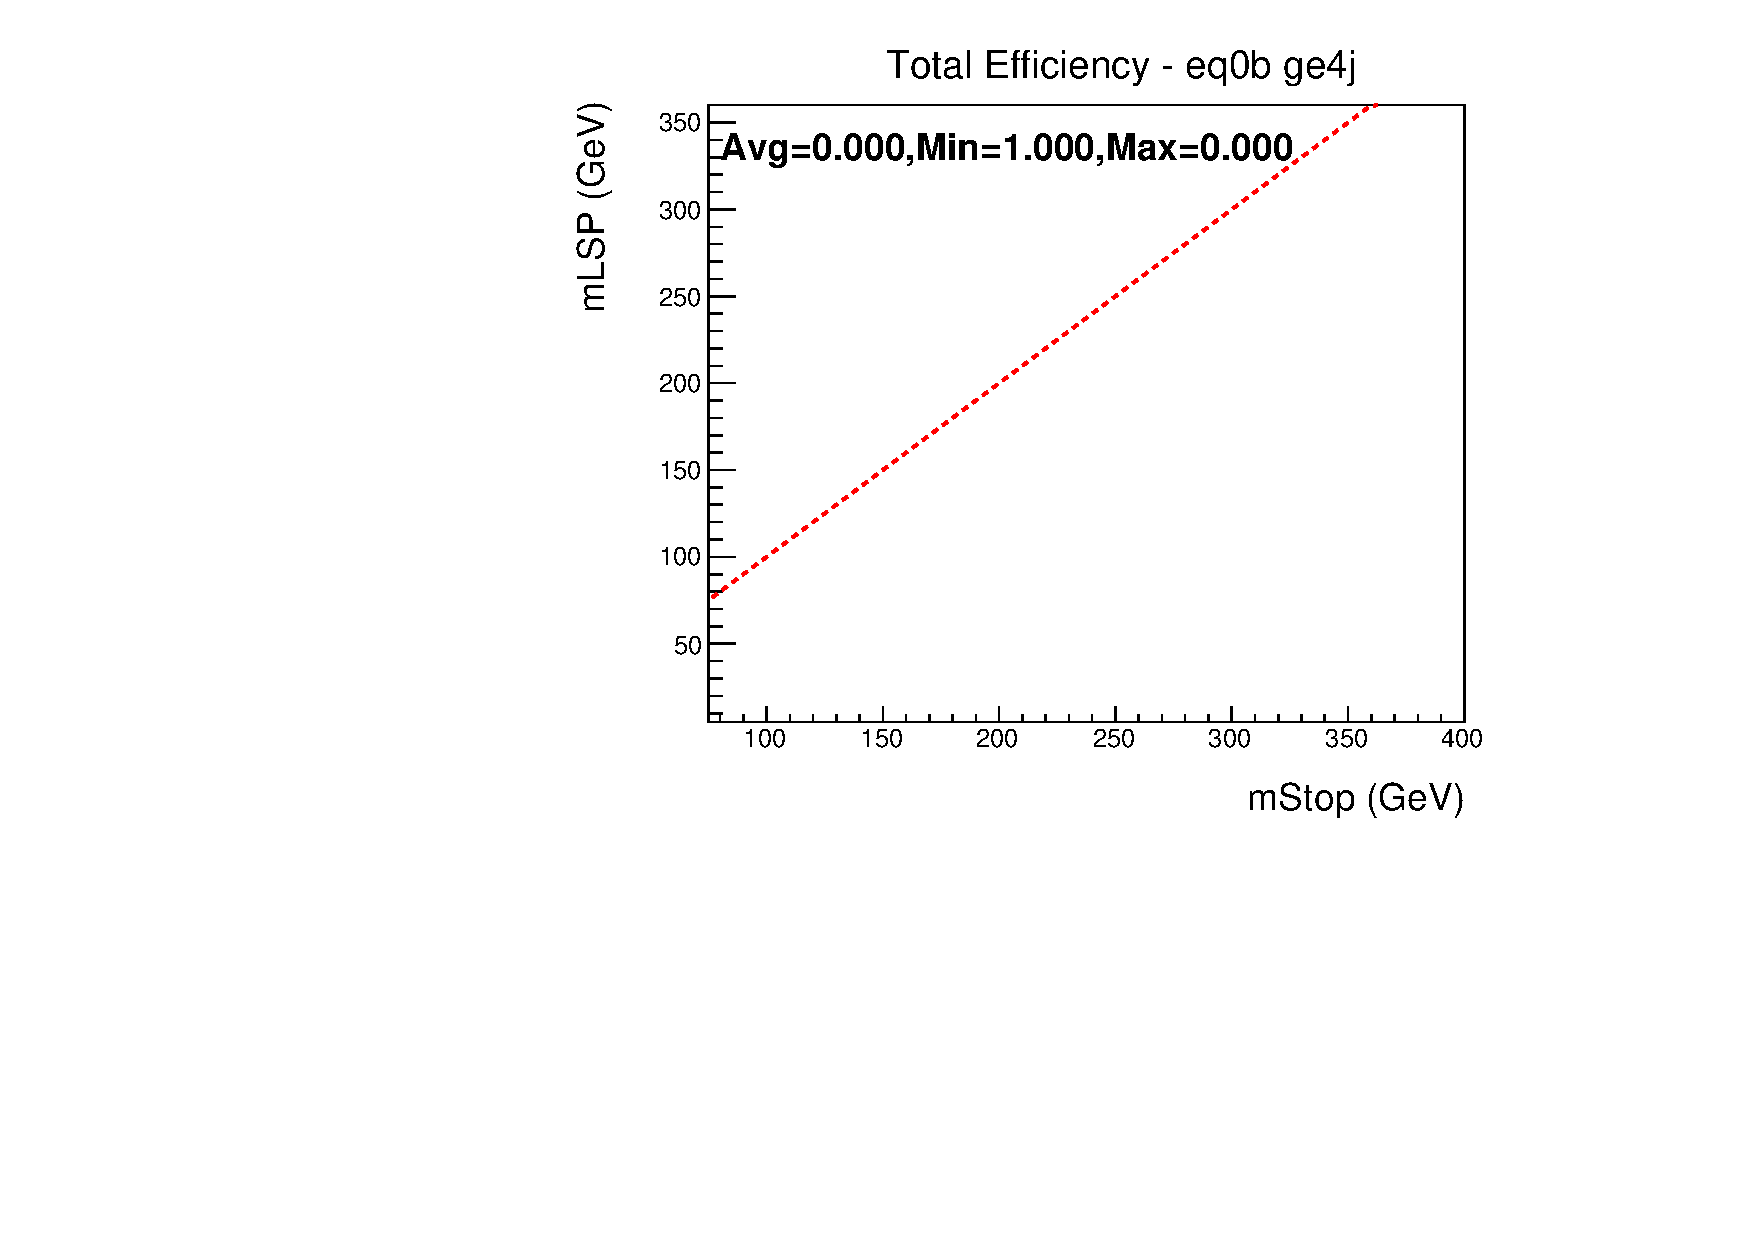
\includegraphics[width=\textwidth]{Figs/sms/t2cc/v24/T2cc_v24_muon_eff_maps_eq0b_ge4j_SITV.pdf}
    \caption{\mj region, ($\geq 4$,0)}
    \label{fig:t2cc_mu_eff_ge4j_0b}
  \end{subfigure} \\
  \begin{subfigure}[b]{0.47\textwidth}
    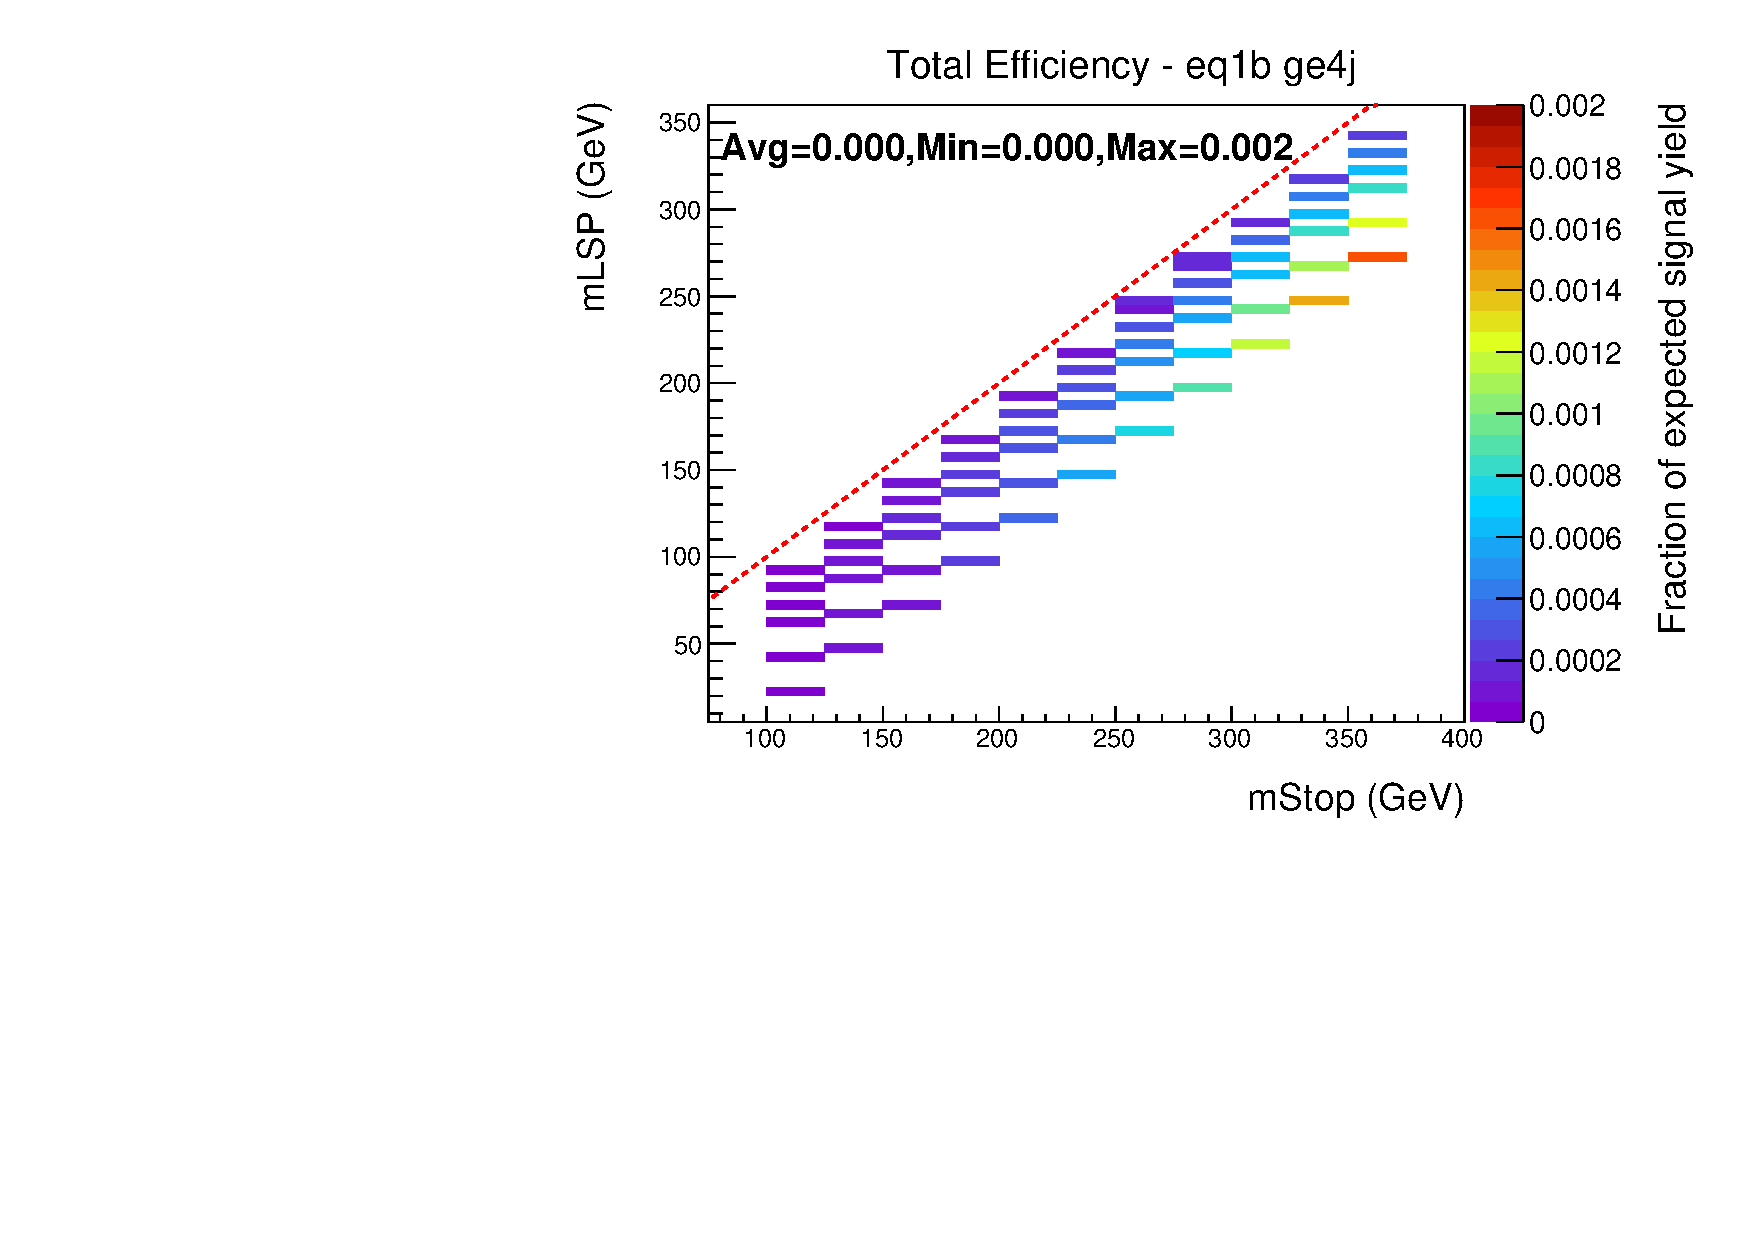
\includegraphics[width=\textwidth]{Figs/sms/t2cc/v24/T2cc_v24_had_eff_maps_eq1b_ge4j_SITV.pdf}
    \caption{Signal region, ($\geq 4$,1)}
    \label{fig:t2cc_sig_eff_ge4j_1b}
  \end{subfigure}
  \begin{subfigure}[b]{0.47\textwidth}
    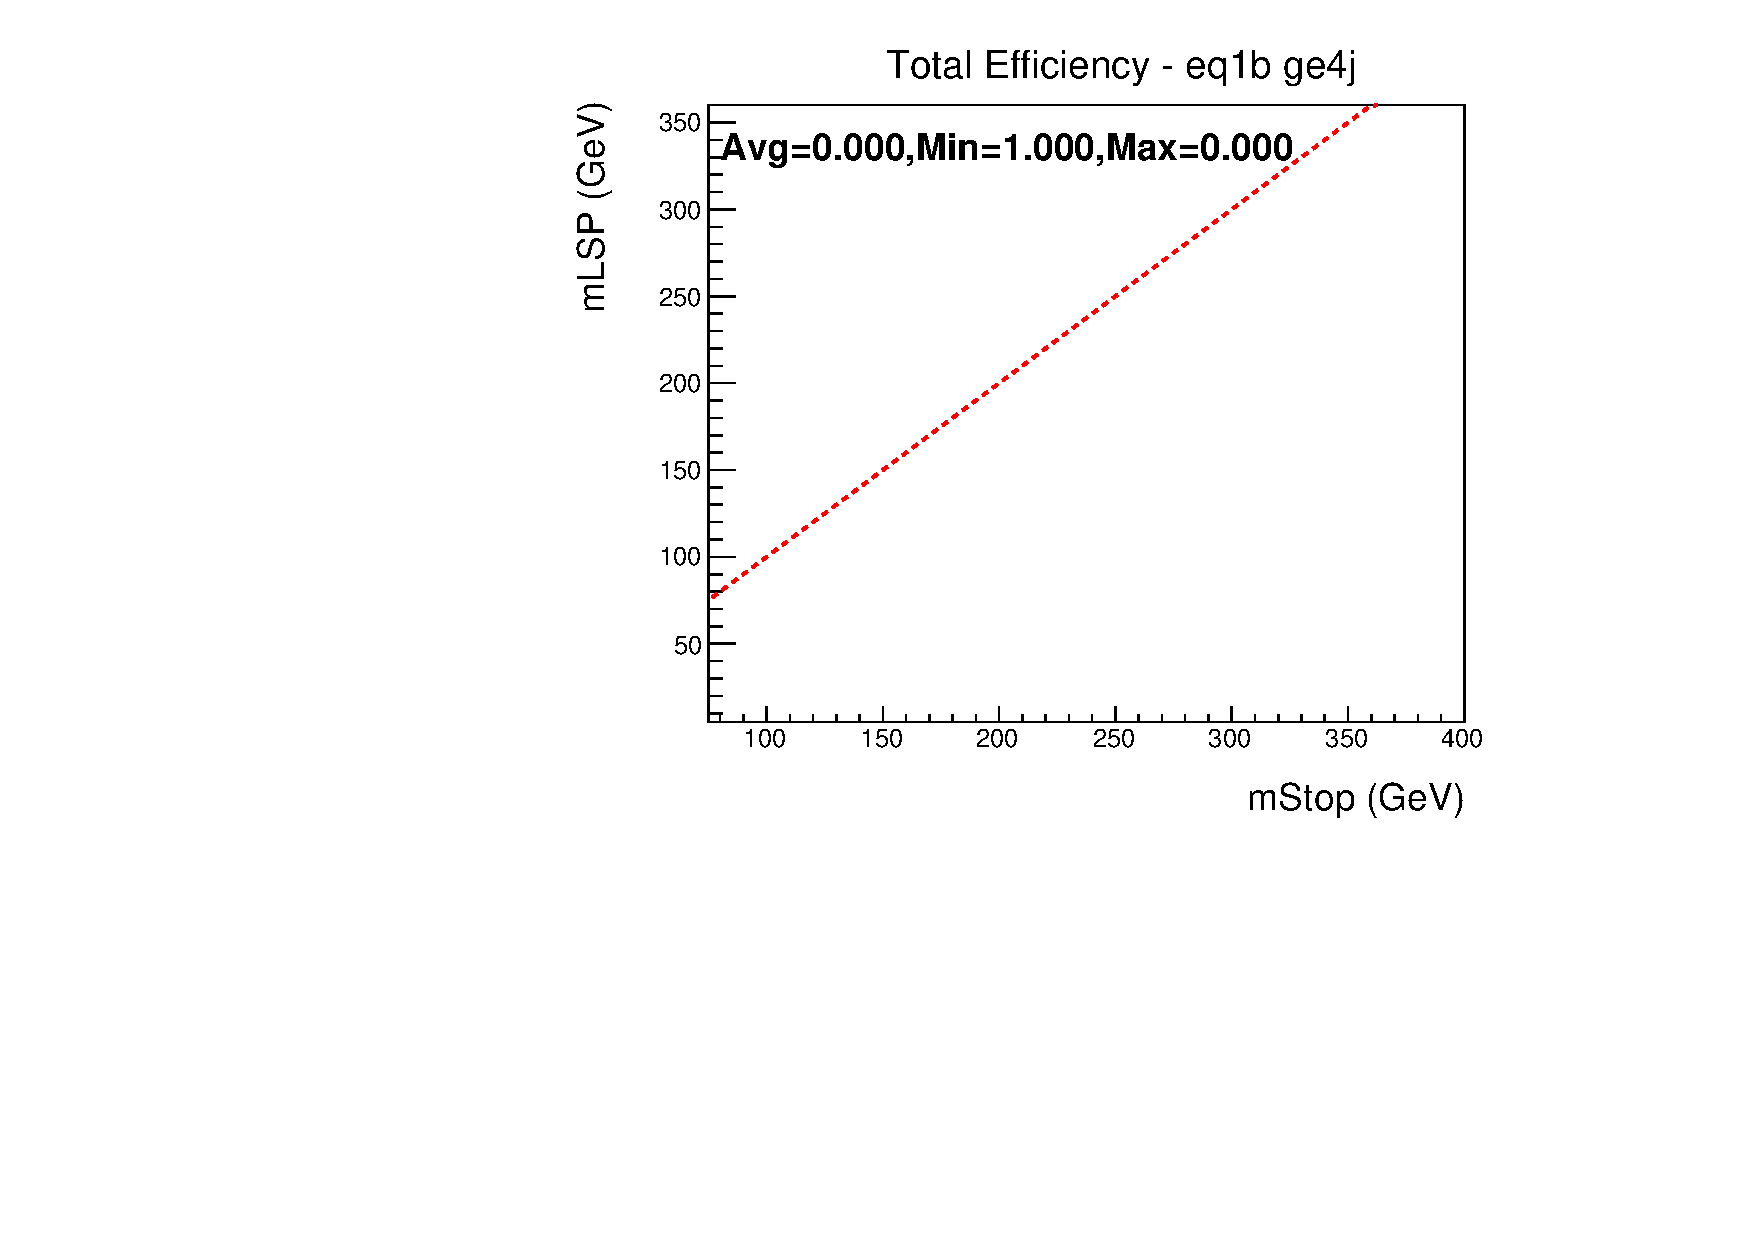
\includegraphics[width=\textwidth]{Figs/sms/t2cc/v24/T2cc_v24_muon_eff_maps_eq1b_ge4j_SITV.pdf}
    \caption{\mj region, ($\geq 4$,1)}
    \label{fig:t2cc_mu_eff_ge4j_1b}
  \end{subfigure} \\
  \caption{Signal efficiency times acceptance for the \Ttwocc simplified, for 
  the hadronic selection (left) and the \mj selection (right), shown for the 
  four most sensitive analysis categories with an inclusive selection on \HT.}
  \label{fig:t2cc_eff}
\end{figure}

% \begin{figure}[h!]
%   \centering
%   \begin{subfigure}[b]{0.6\textwidth}
%     \includegraphics[width=\textwidth, trim=0 0 0 30, clip=true]{Figs/sms/t2cc/v24/T2cc_v24_sig_inj_250_170.pdf}
%     \caption{$m_{\sTop} = 250\gev, m_{\rm LSP} = 170\gev$}
%     \label{fig:t2cc_sig_inj_dm80}
%   \end{subfigure}
%   \begin{subfigure}[b]{0.6\textwidth}
%     \includegraphics[width=\textwidth, trim=0 0 0 30, clip=true]{Figs/sms/t2cc/v24/T2cc_v24_sig_inj_250_240.pdf}
%     \caption{$m_{\sTop} = 250\gev, m_{\rm LSP} = 240\gev$}
%     \label{fig:t2cc_sig_inj_dm10}
%   \end{subfigure}
%   \caption{balls}
%   \label{fig:}
% \end{figure}

\subsection{T2\_4body}

The \Ttwodegen model signal efficiency times acceptance distributions are shown 
in figure~\ref{fig:t2_4body_eff} in the four most sensitive analysis categories,
with an inclusive \HT selection, both for the hadronic and \mj selections. There
are strong similarities with those shown earlier for the \texttt{T2cc} model, 
both in magnitude and distribution about the plane. At small values of \deltam, 
given that the entire susy decay system becomes invisible due to a lack of 
kinematic phase space, both models show very similar efficiencies, where 
acceptance is almost entirely due to hard ISR jets within acceptance. There is a
significant difference however, when a b-tagged jet is required, for example in 
the \njlow, \nb=1 category, where the presence of a jet originating from a real 
b quark improves acceptance, particularly away from the diagonal where this jet 
would be more likely to pass analysis thresholds. Less significant are the 
efficiencies seen in the \njhigh categories, given the larger number of final 
state object, each requiring a share of the energy originating from the mass 
splitting of the mother and daughter sparticles.

Also of note is the increase in signal contamination observed in the \mj 
selection, due to the presence of $f\bar{f}$ in the decay chain, potentially 
giving leptons in the final state.

% should be v16!!
\begin{figure}[ht!]
  \centering
  \begin{subfigure}[b]{0.47\textwidth}
    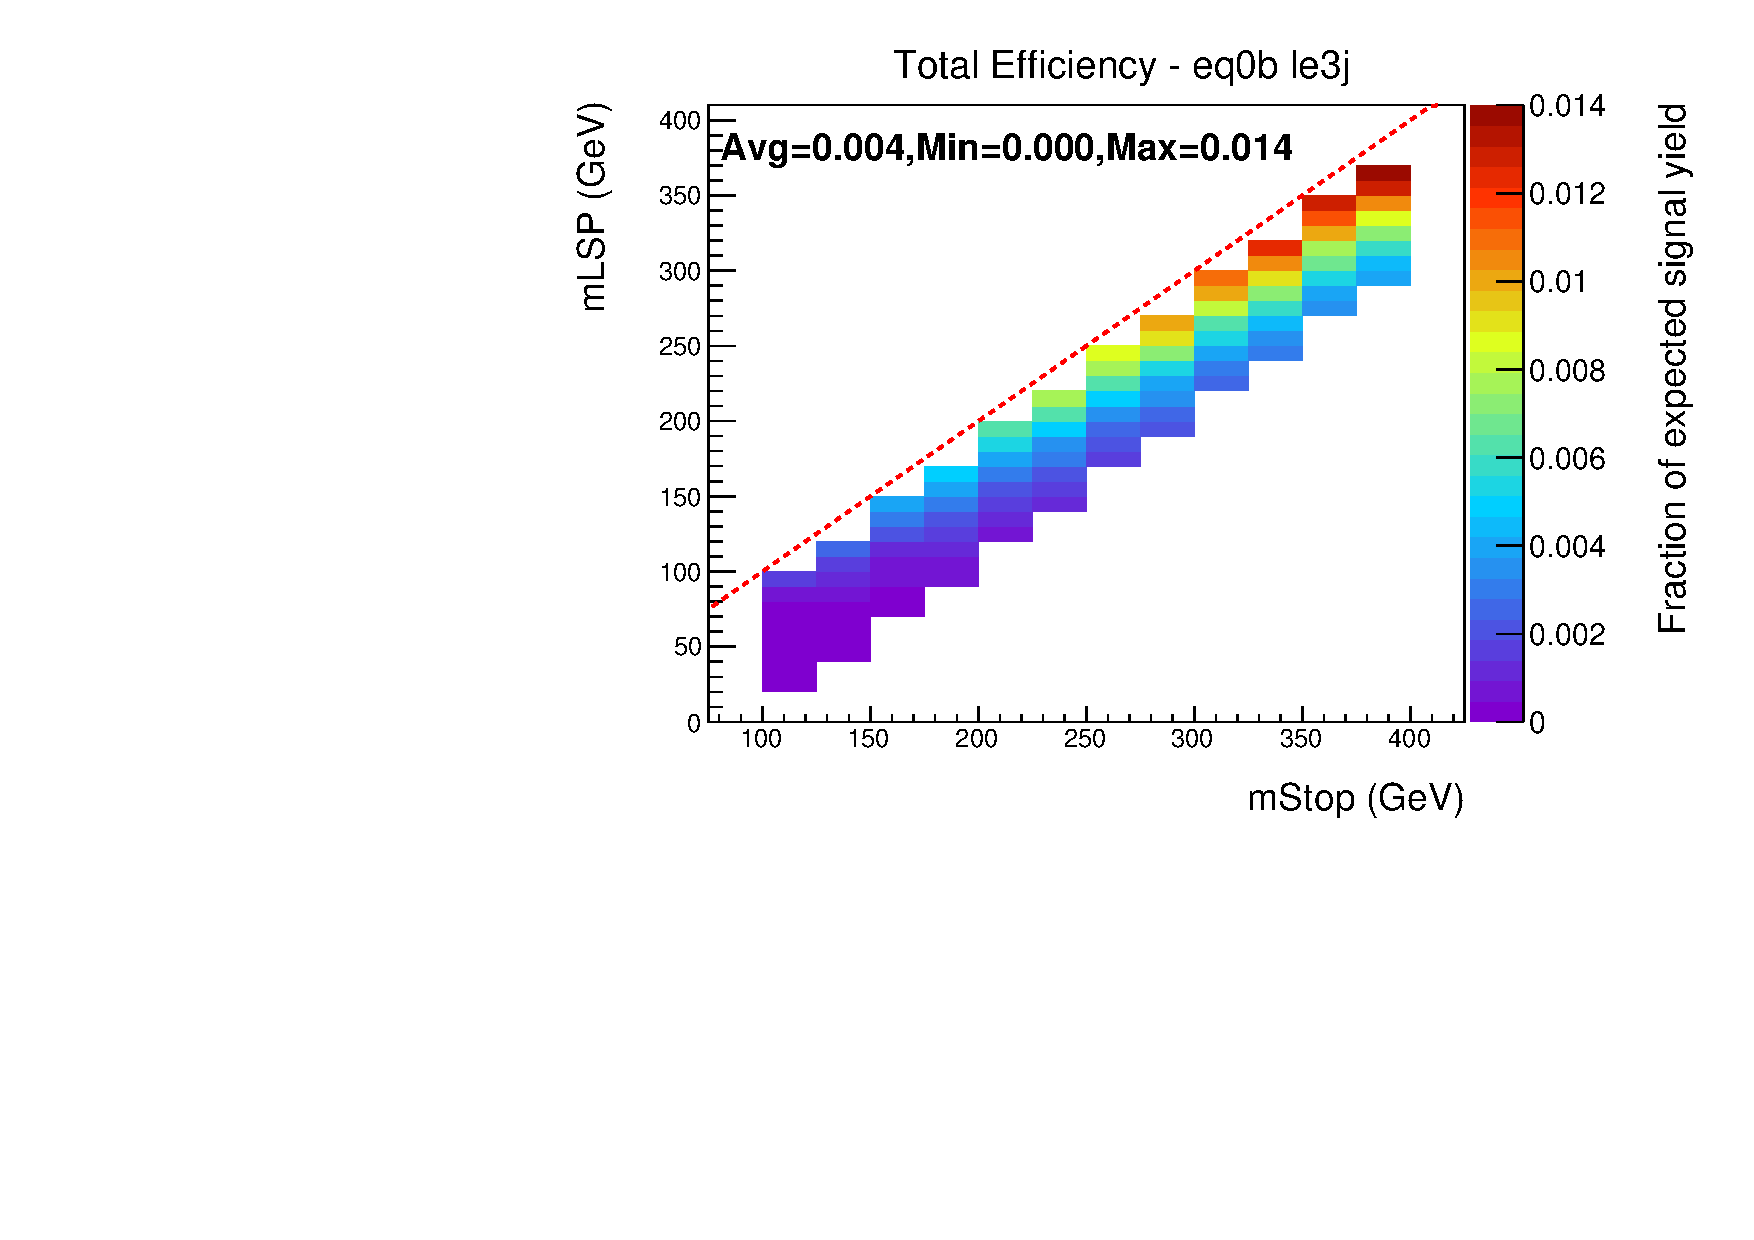
\includegraphics[width=\textwidth]{Figs/sms/t2degen/v5/T2_4body_v5_had_eff_maps_eq0b_le3j_SITV.pdf}
    \caption{Signal region, (2--3,0)}
    \label{fig:t2_4body_sig_eff_le3j_0b}
  \end{subfigure}
  \begin{subfigure}[b]{0.47\textwidth}
    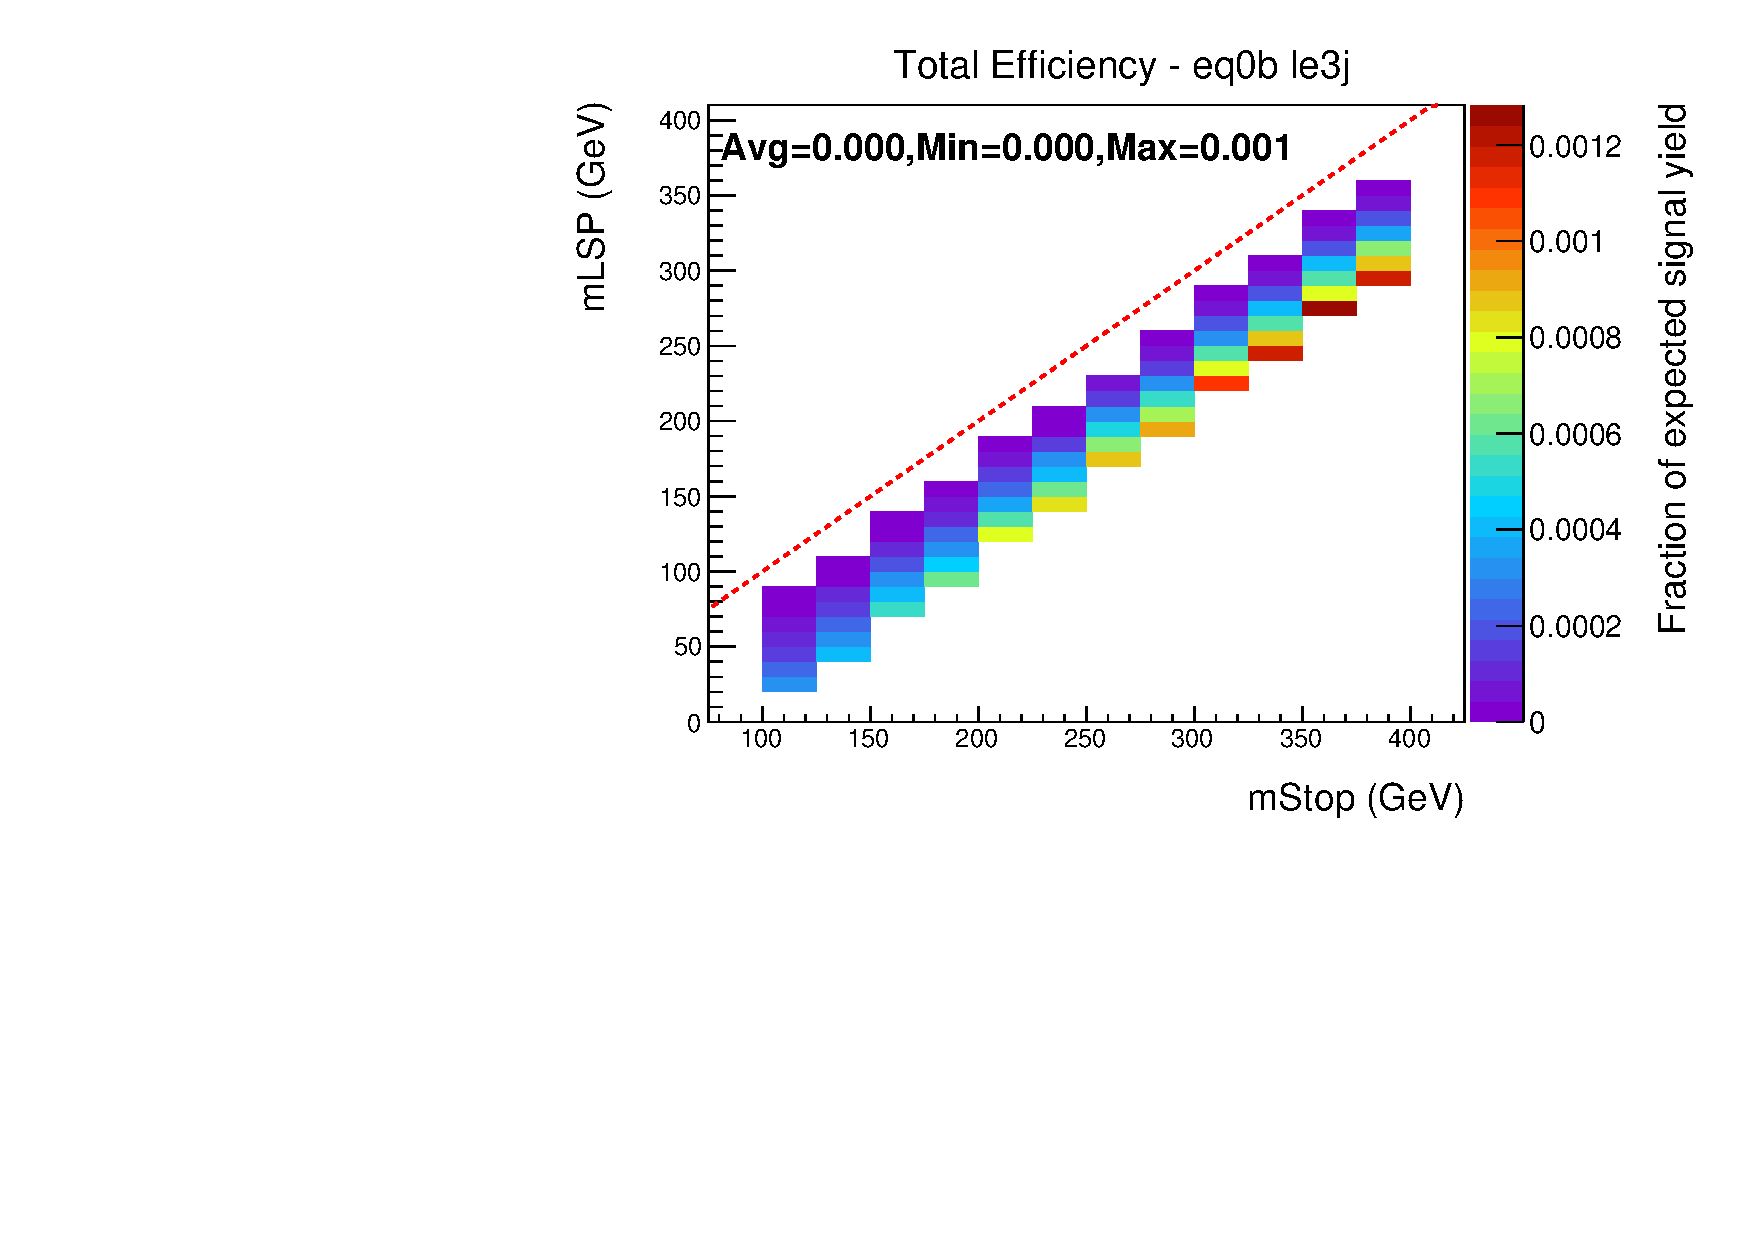
\includegraphics[width=\textwidth]{Figs/sms/t2degen/v5/T2_4body_v5_muon_eff_maps_eq0b_le3j_SITV.pdf}
    \caption{\mj region, (2--3,0)}
    \label{fig:t2_4body_mu_eff_le3j_0b}
  \end{subfigure} \\
  \begin{subfigure}[b]{0.47\textwidth}
    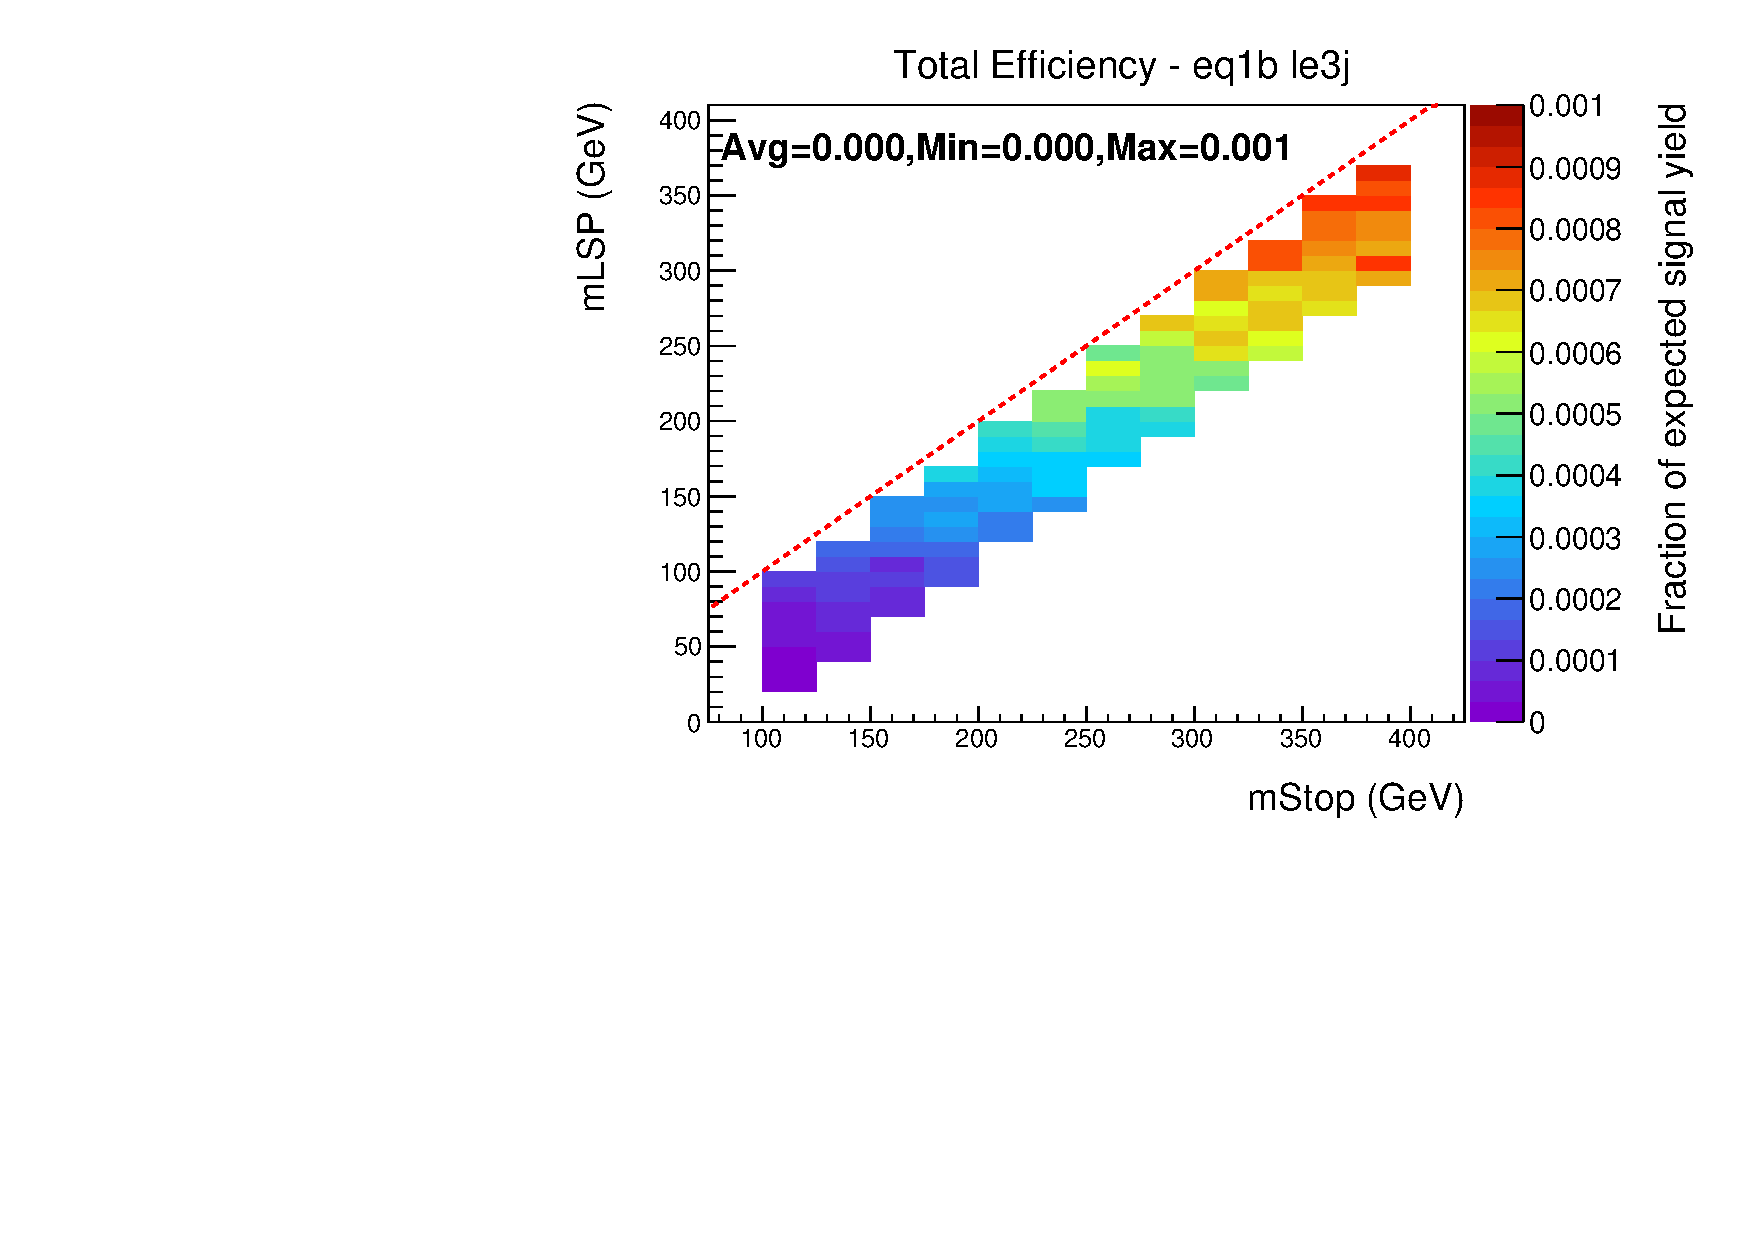
\includegraphics[width=\textwidth]{Figs/sms/t2degen/v5/T2_4body_v5_had_eff_maps_eq1b_le3j_SITV.pdf}
    \caption{Signal region, (2--3,1)}
    \label{fig:t2_4body_sig_eff_le3j_1b}
  \end{subfigure}
  \begin{subfigure}[b]{0.47\textwidth}
    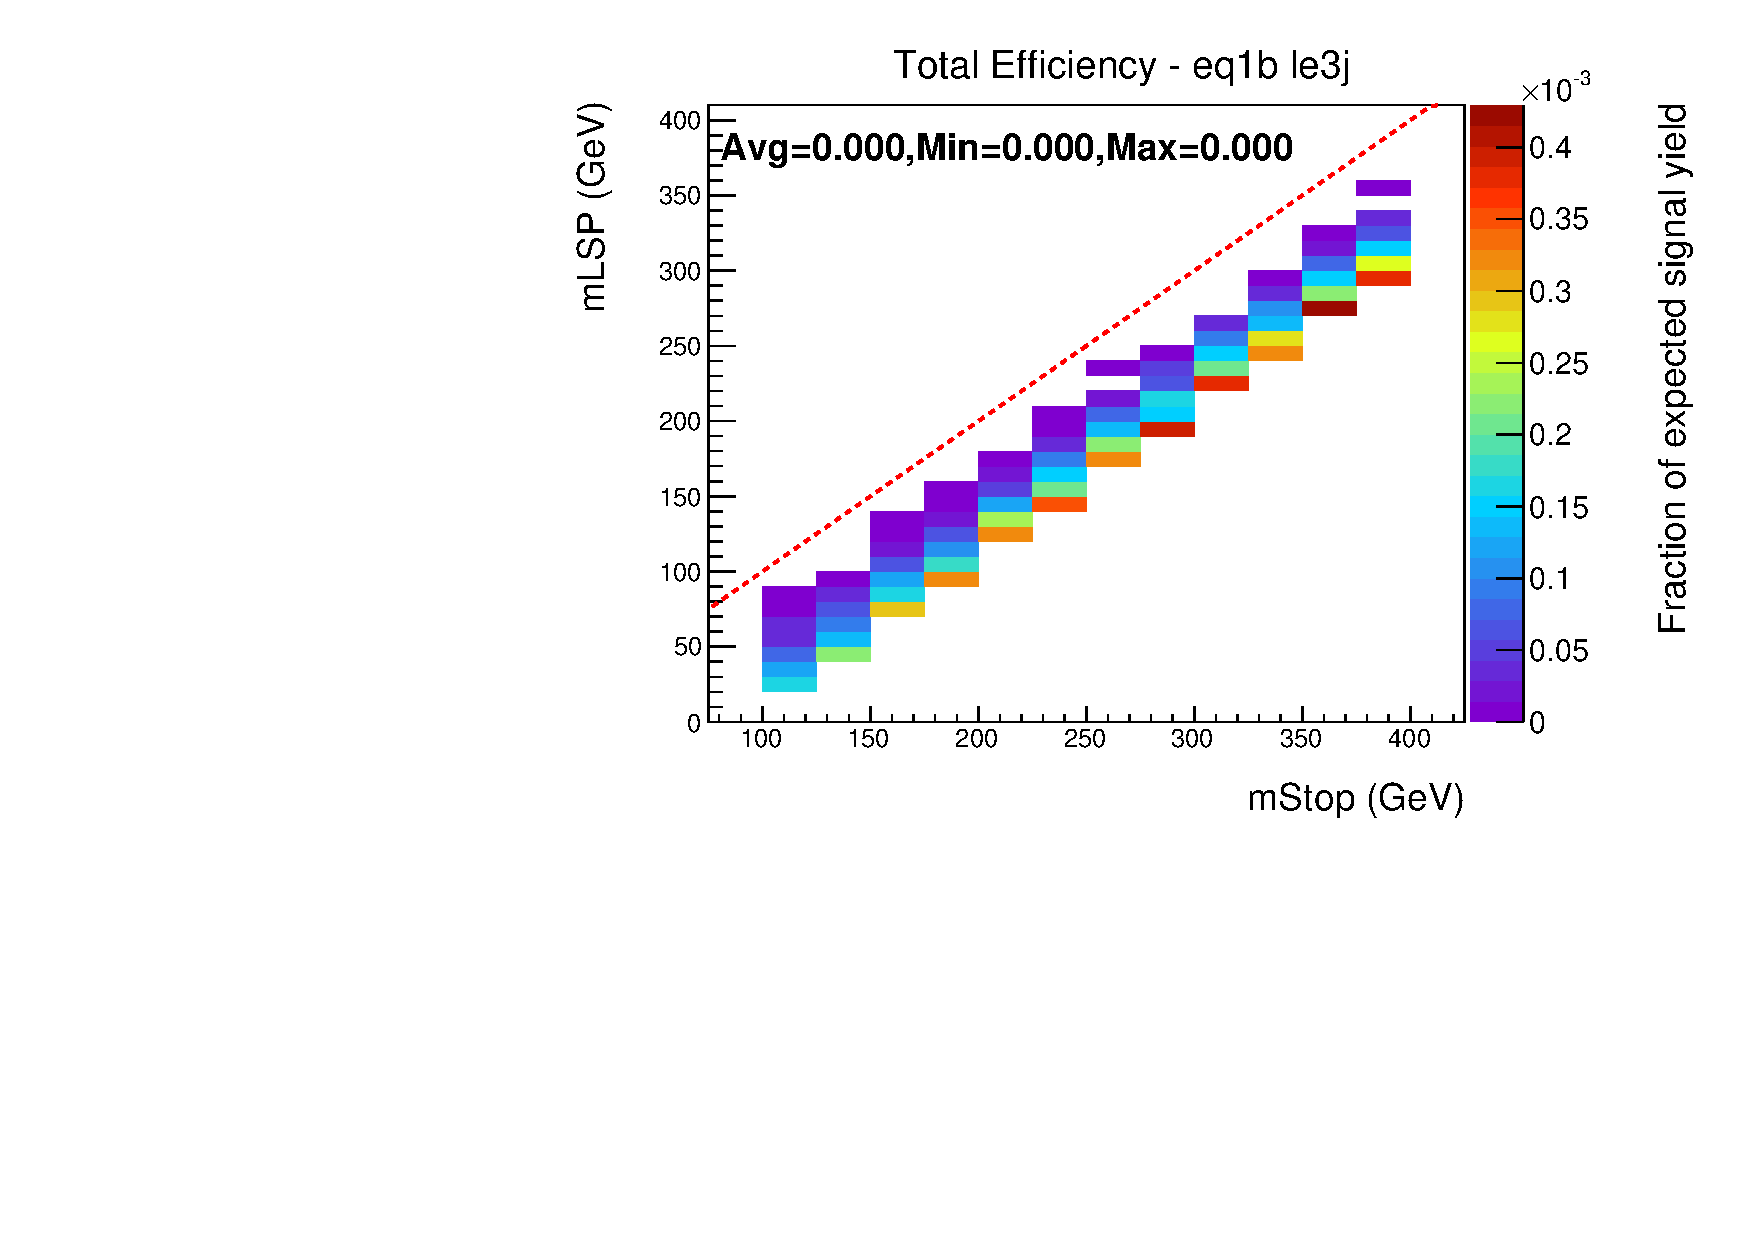
\includegraphics[width=\textwidth]{Figs/sms/t2degen/v5/T2_4body_v5_muon_eff_maps_eq1b_le3j_SITV.pdf}
    \caption{\mj region, (2--3,1)}
    \label{fig:t2_4body_mu_eff_le3j_1b}
  \end{subfigure} \\
  \begin{subfigure}[b]{0.47\textwidth}
    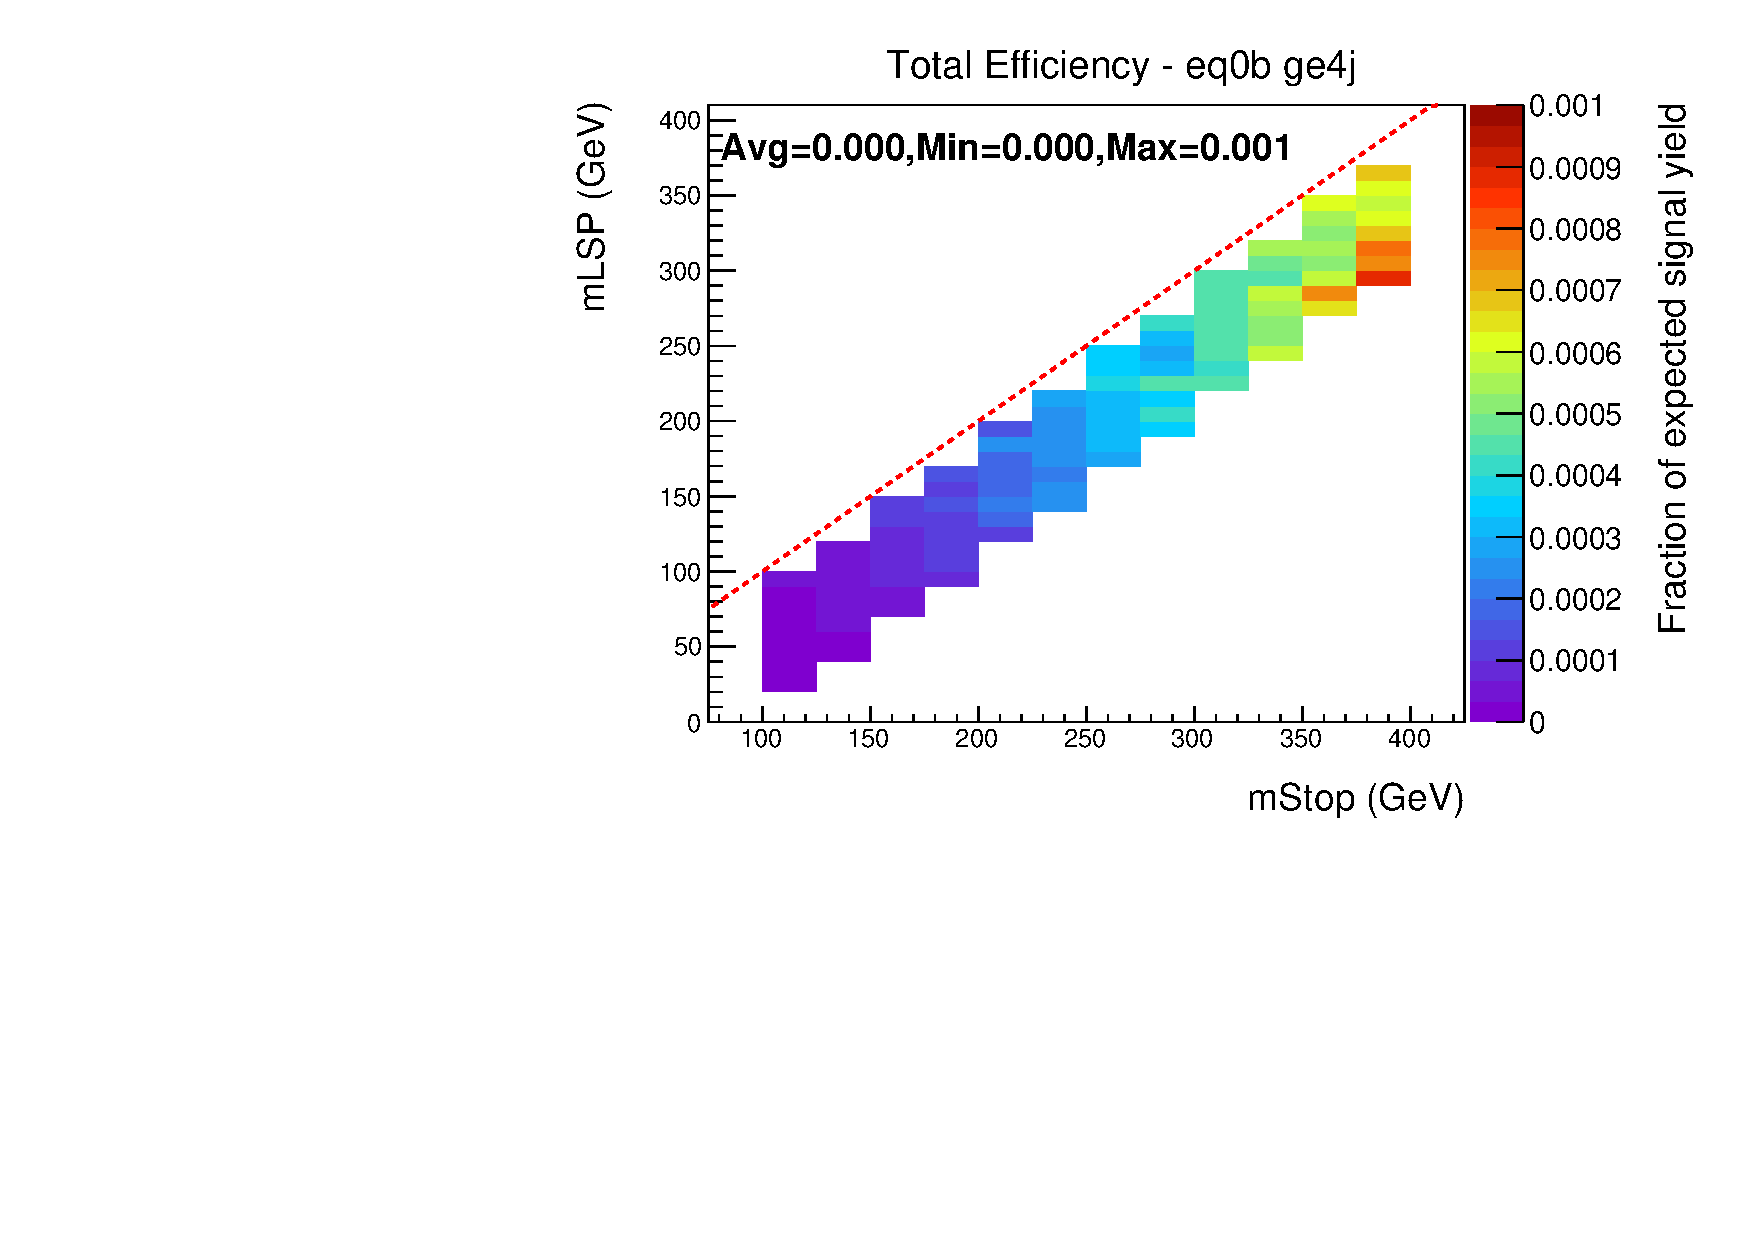
\includegraphics[width=\textwidth]{Figs/sms/t2degen/v5/T2_4body_v5_had_eff_maps_eq0b_ge4j_SITV.pdf}
    \caption{Signal region, ($\geq 4$,0)}
    \label{fig:t2_4body_sig_eff_ge4j_0b}
  \end{subfigure}
  \begin{subfigure}[b]{0.47\textwidth}
    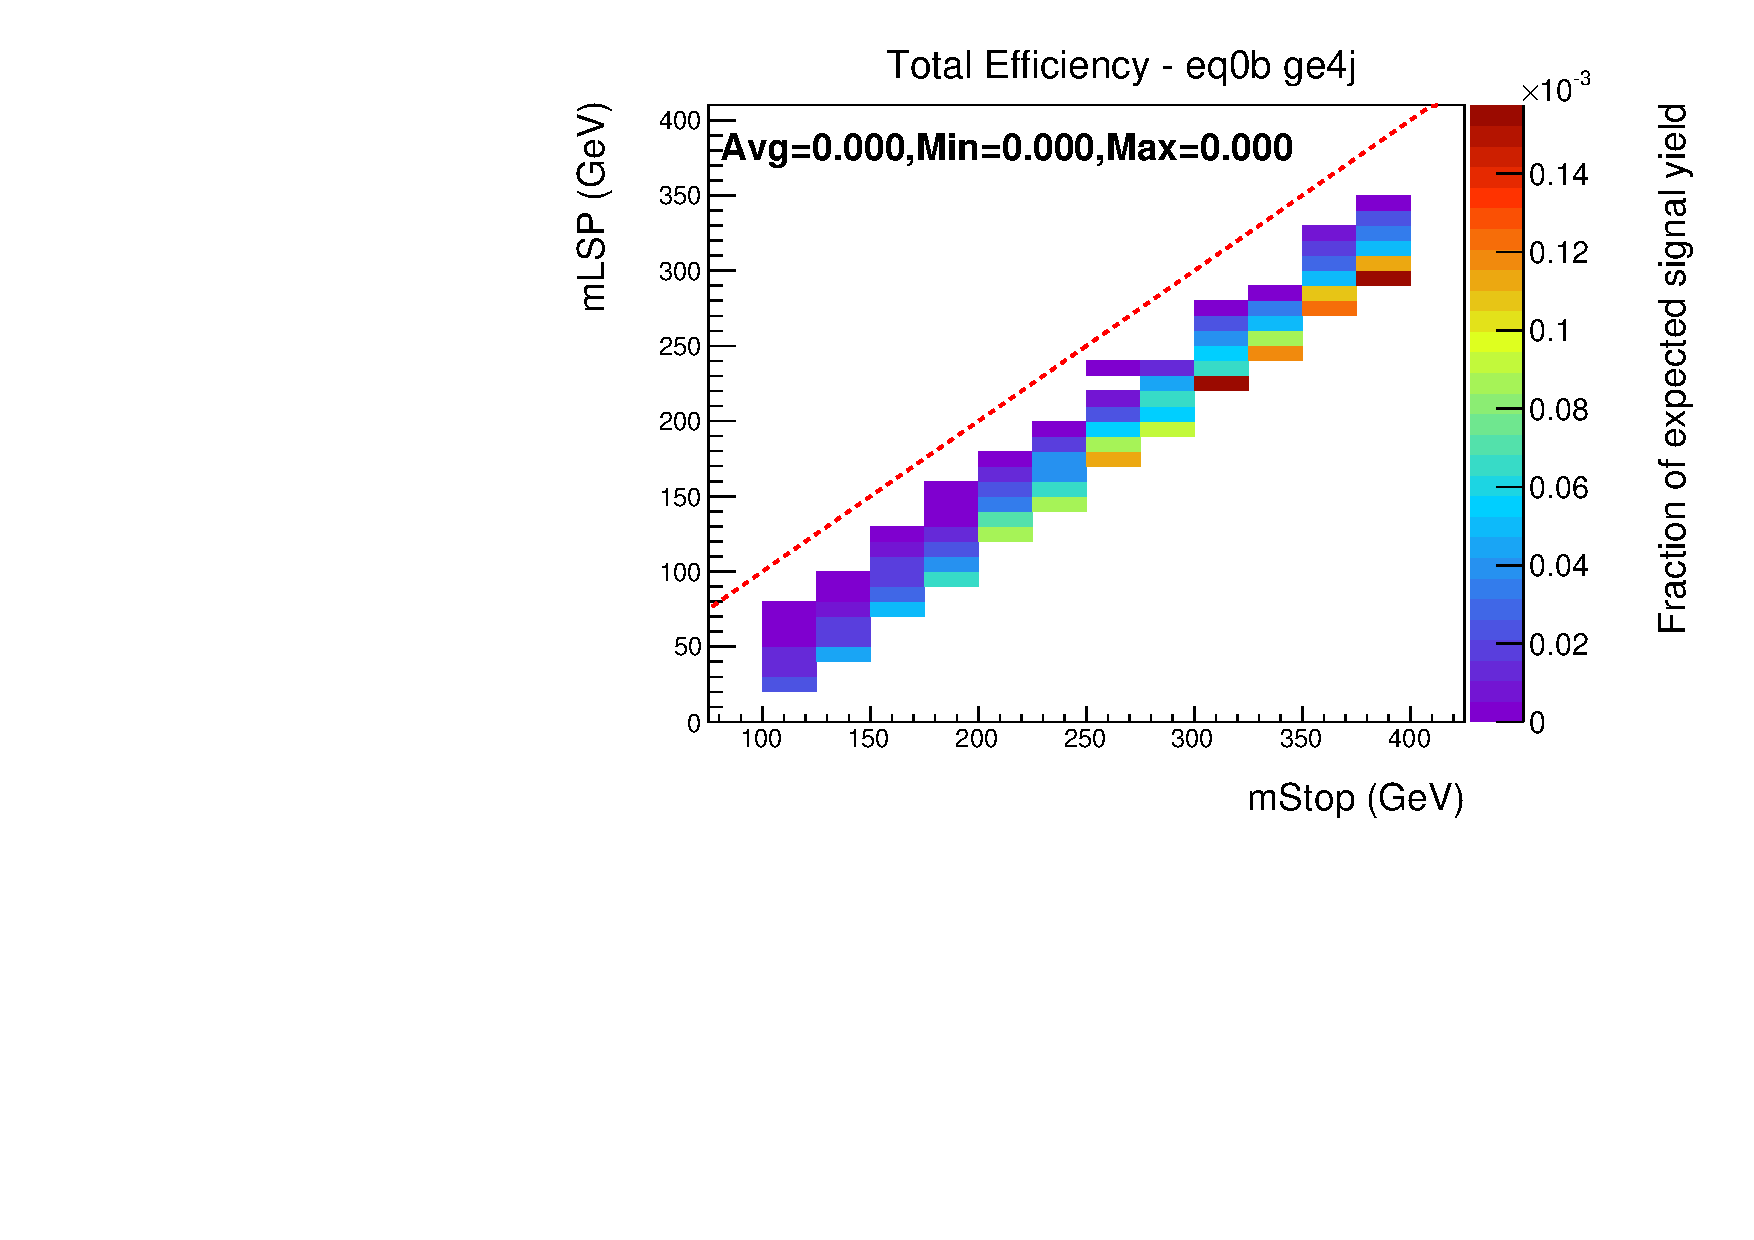
\includegraphics[width=\textwidth]{Figs/sms/t2degen/v5/T2_4body_v5_muon_eff_maps_eq0b_ge4j_SITV.pdf}
    \caption{\mj region, ($\geq 4$,0)}
    \label{fig:t2_4body_mu_eff_ge4j_0b}
  \end{subfigure} \\
  \begin{subfigure}[b]{0.47\textwidth}
    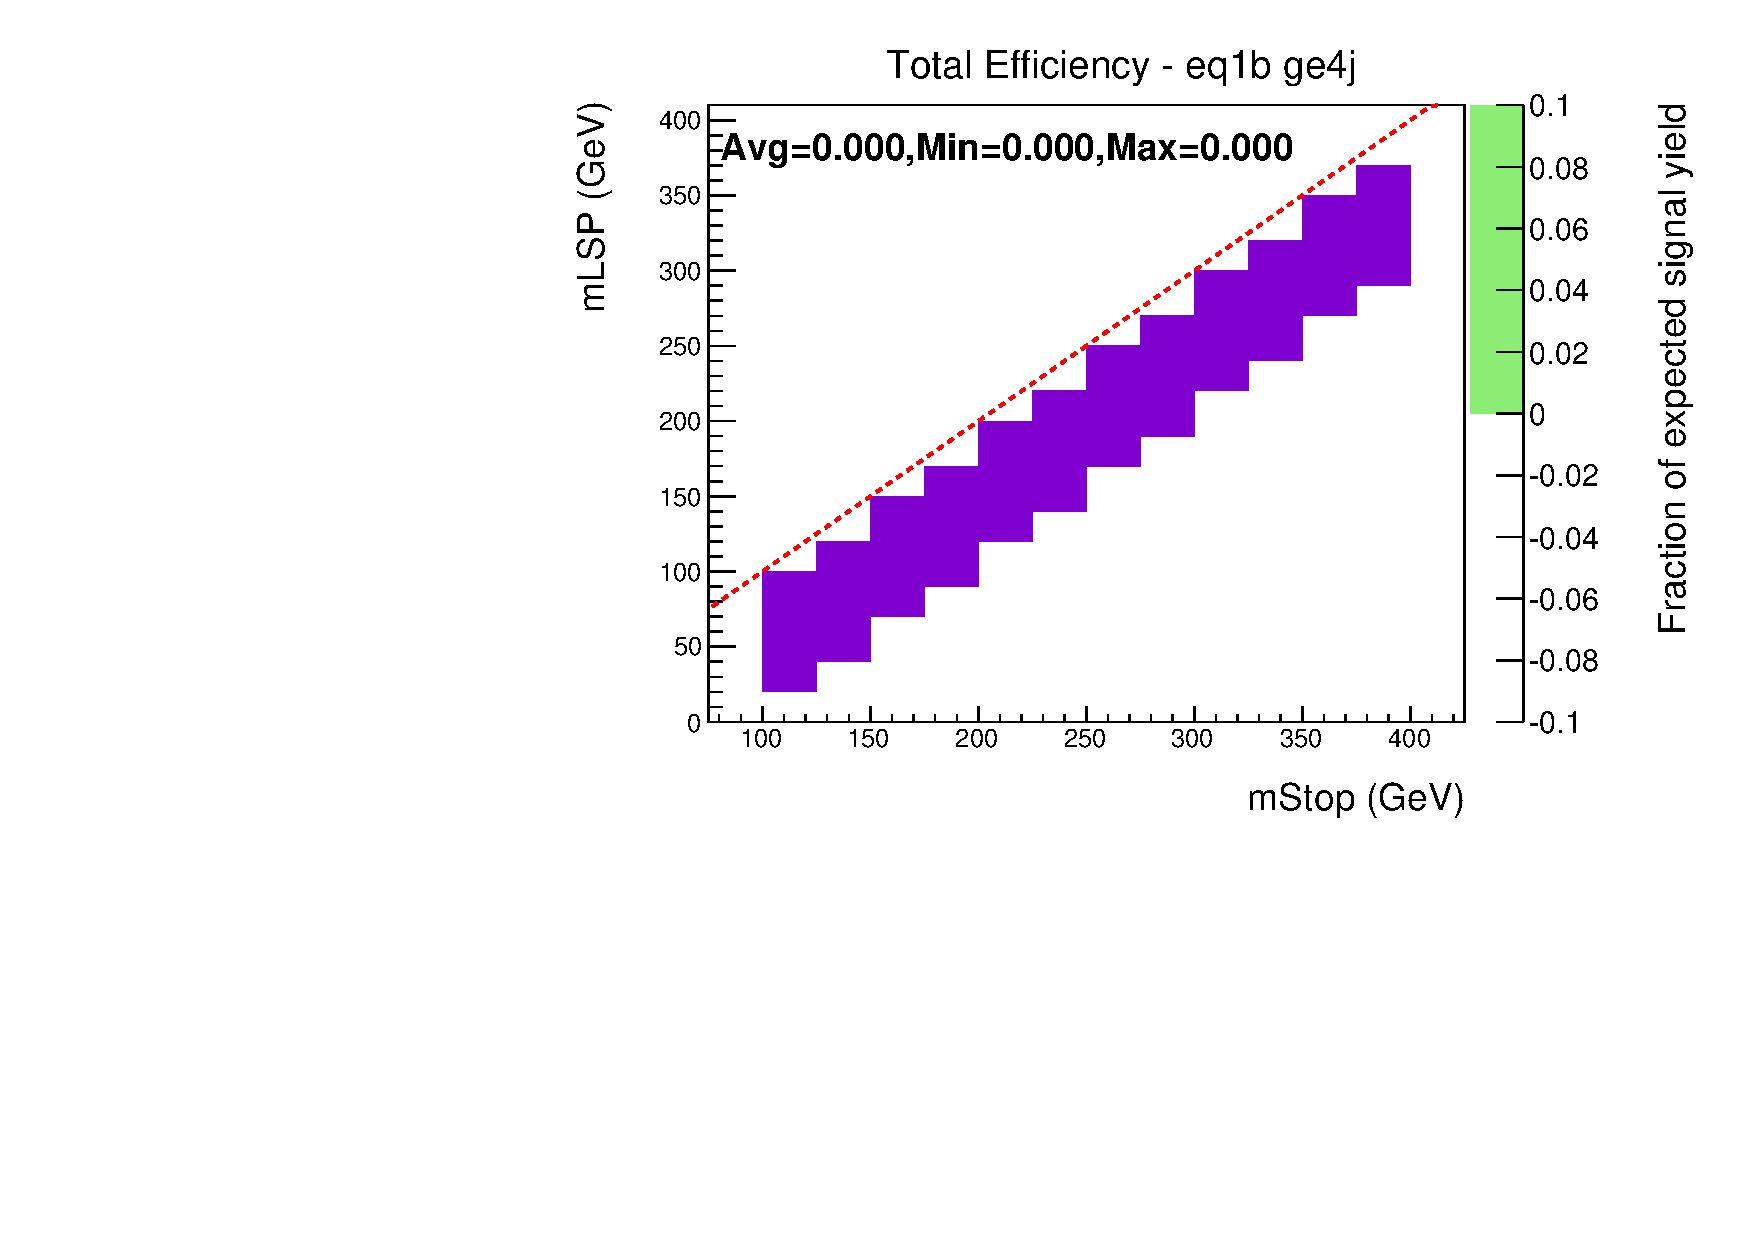
\includegraphics[width=\textwidth]{Figs/sms/t2degen/v5/T2_4body_v5_had_eff_maps_eq1b_ge4j_SITV.pdf}
    \caption{Signal region, ($\geq 4$,1)}
    \label{fig:t2_4body_sig_eff_ge4j_1b}
  \end{subfigure}
  \begin{subfigure}[b]{0.47\textwidth}
    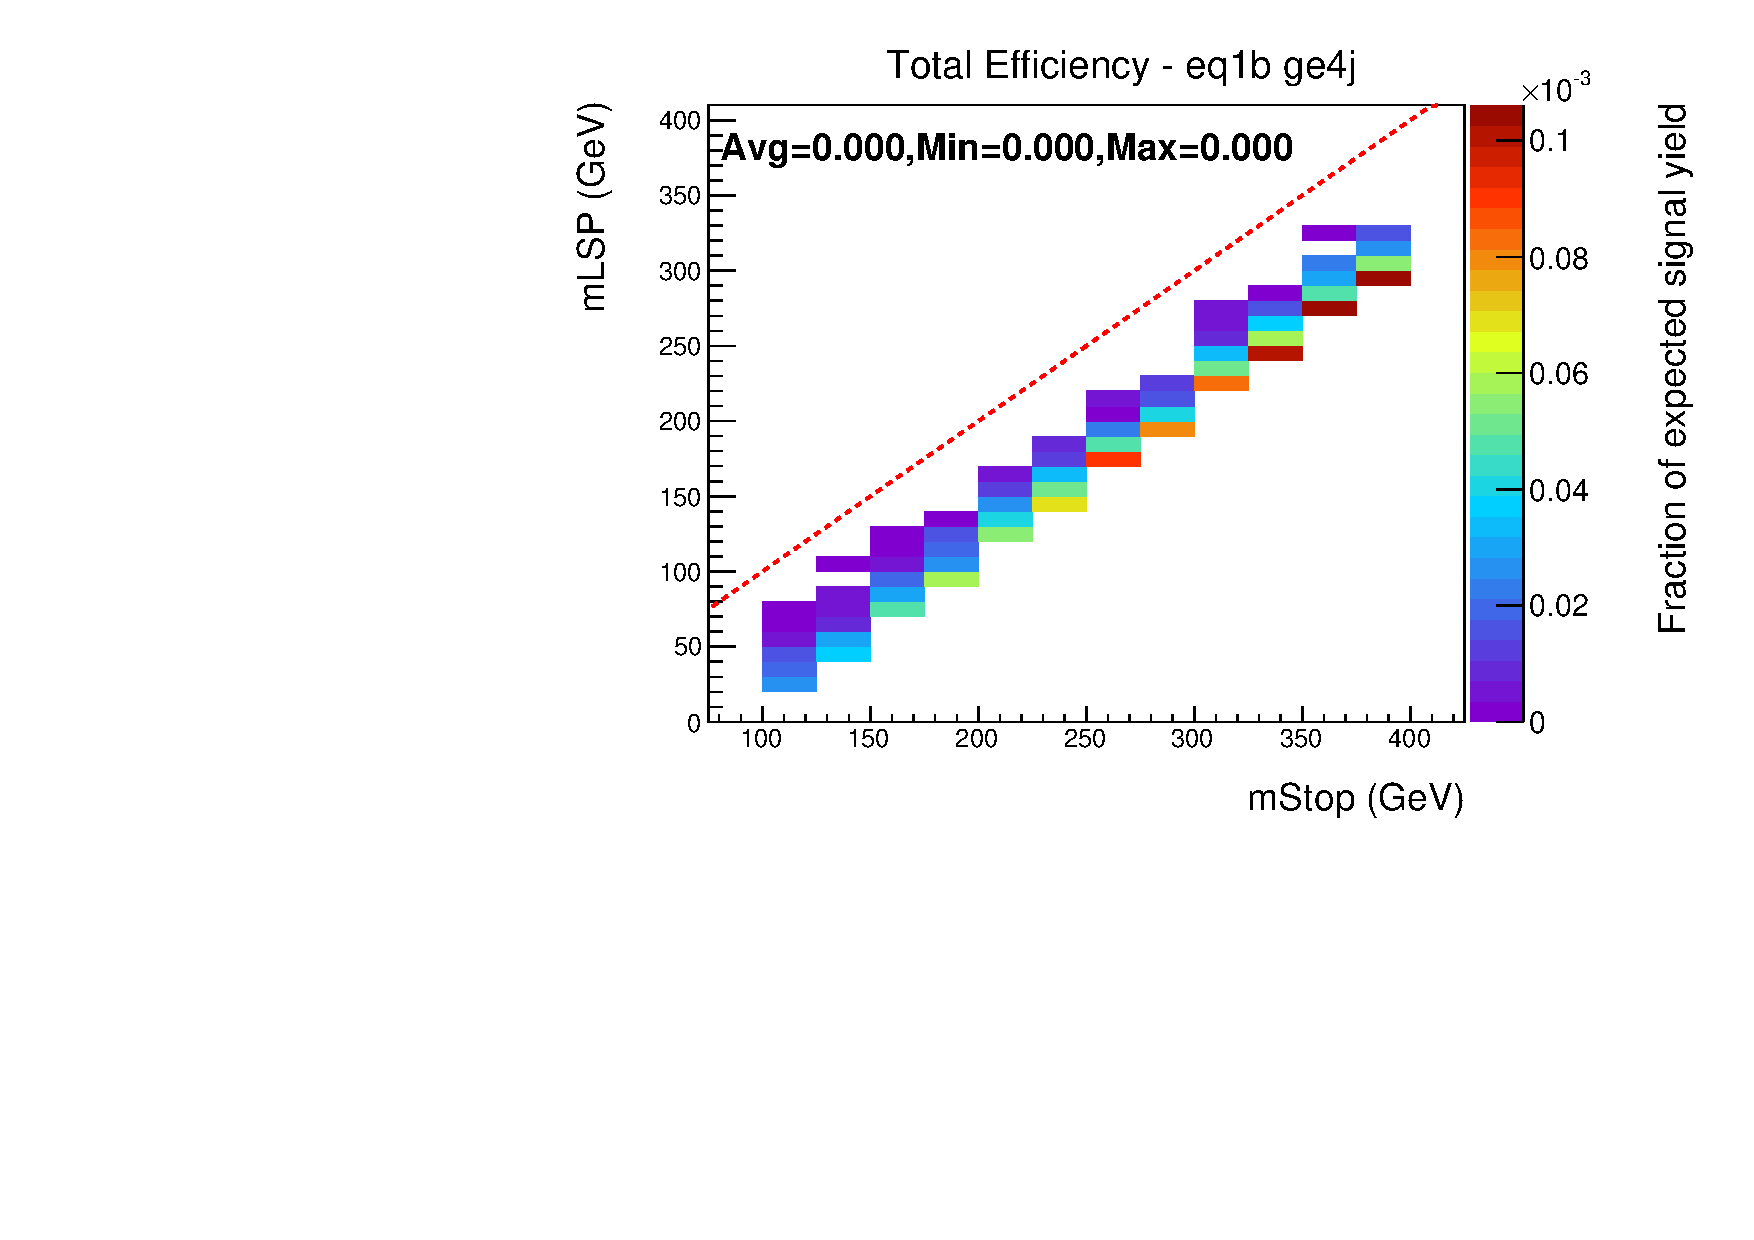
\includegraphics[width=\textwidth]{Figs/sms/t2degen/v5/T2_4body_v5_muon_eff_maps_eq1b_ge4j_SITV.pdf}
    \caption{\mj region, ($\geq 4$,1)}
    \label{fig:t2_4body_mu_eff_ge4j_1b}
  \end{subfigure} \\
  \caption{Signal efficiency times acceptance for the \Ttwodegen simplified, for 
  the hadronic selection (left) and the \mj selection (right), shown for the 
  four most sensitive analysis categories with an inclusive selection on \HT.}
  \label{fig:t2_4body_eff}
\end{figure}


% \begin{figure}[!h]
%  \begin{center}
%    \subfigure[Signal region, (2--3,0)]{
%      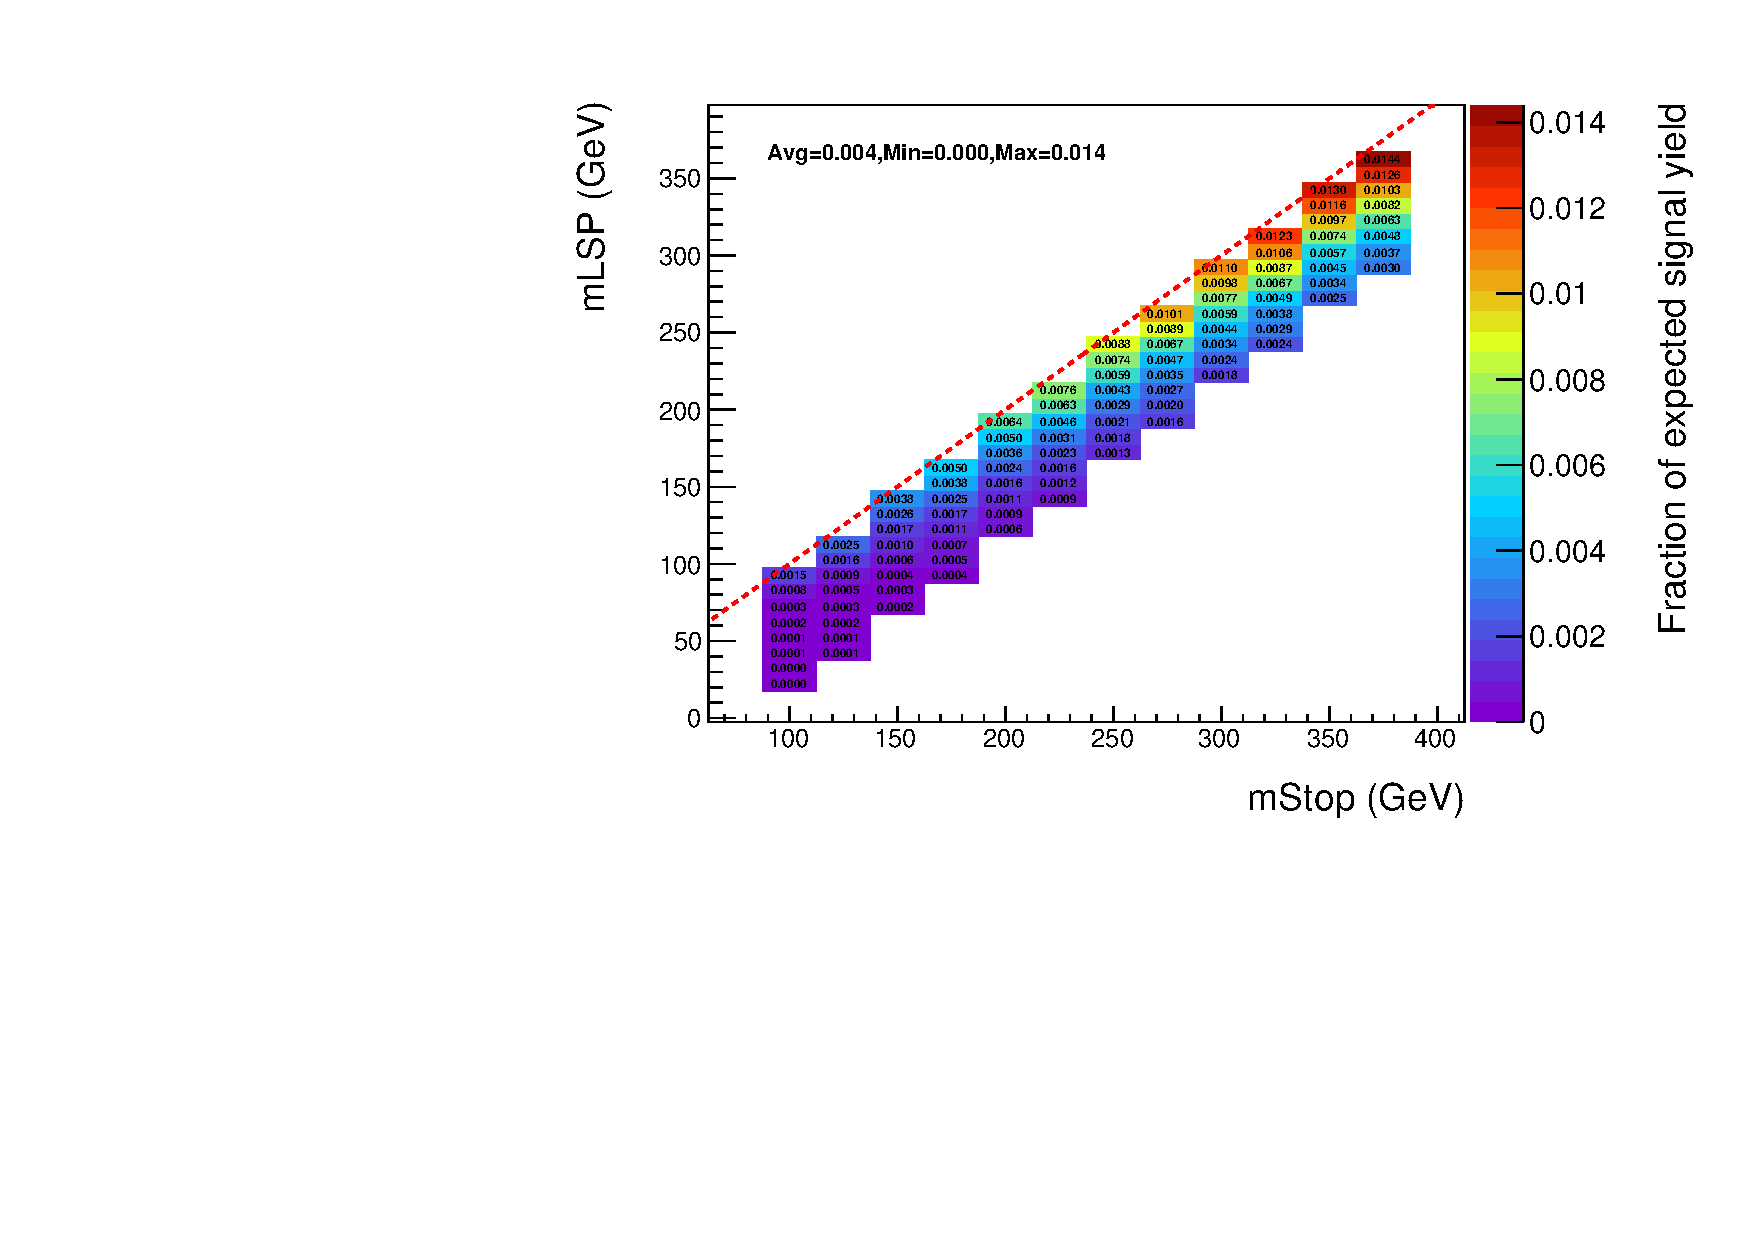
\includegraphics[width=0.4\textwidth]{figures/sms/t2_4body/v16/T2_4body_had_eff_maps_eq0b_le3j_SITV}
%    } 
%    \subfigure[\mj sample, (2--3,0)]{
%      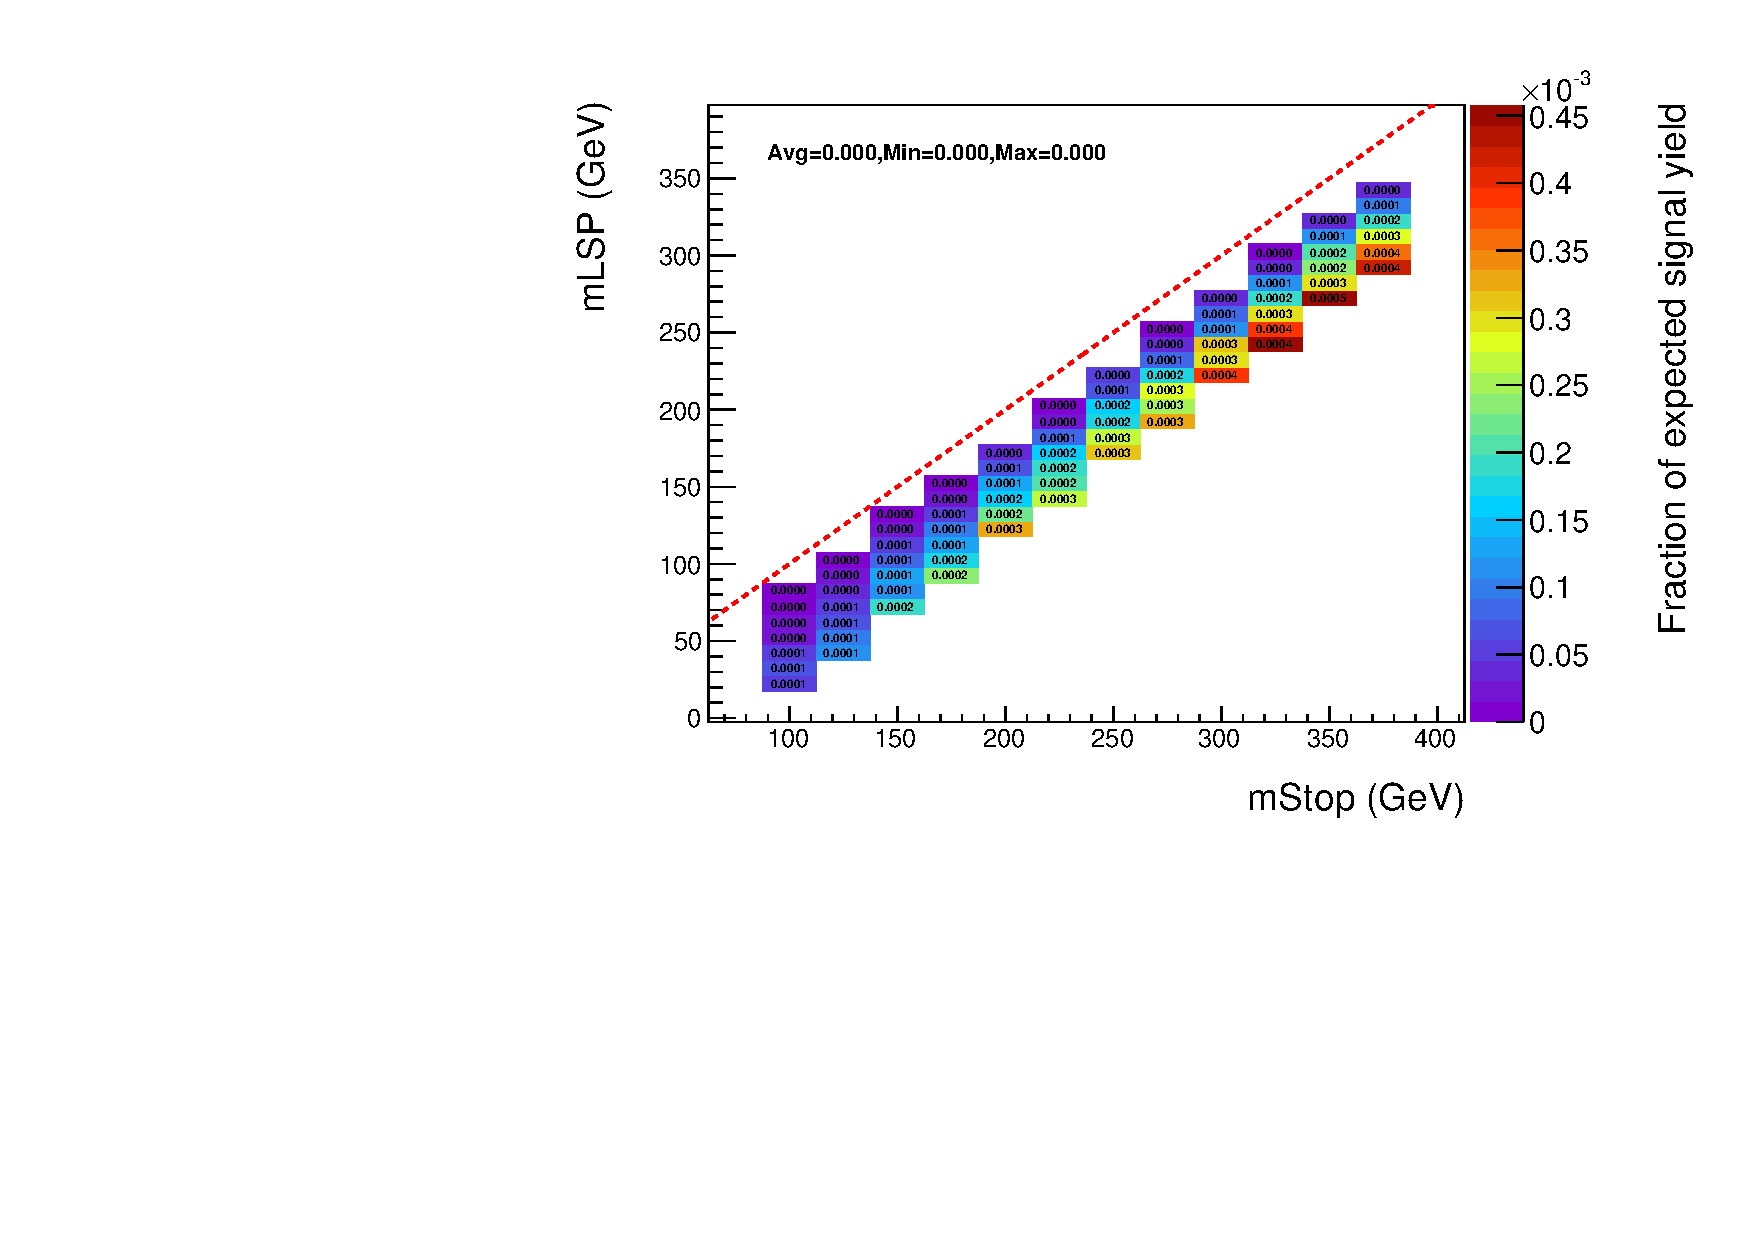
\includegraphics[width=0.4\textwidth]{figures/sms/t2_4body/v16/T2_4body_muon_eff_maps_eq0b_le3j_SITV}
%    } \\
%    \subfigure[Signal region, (2--3,1)]{
%      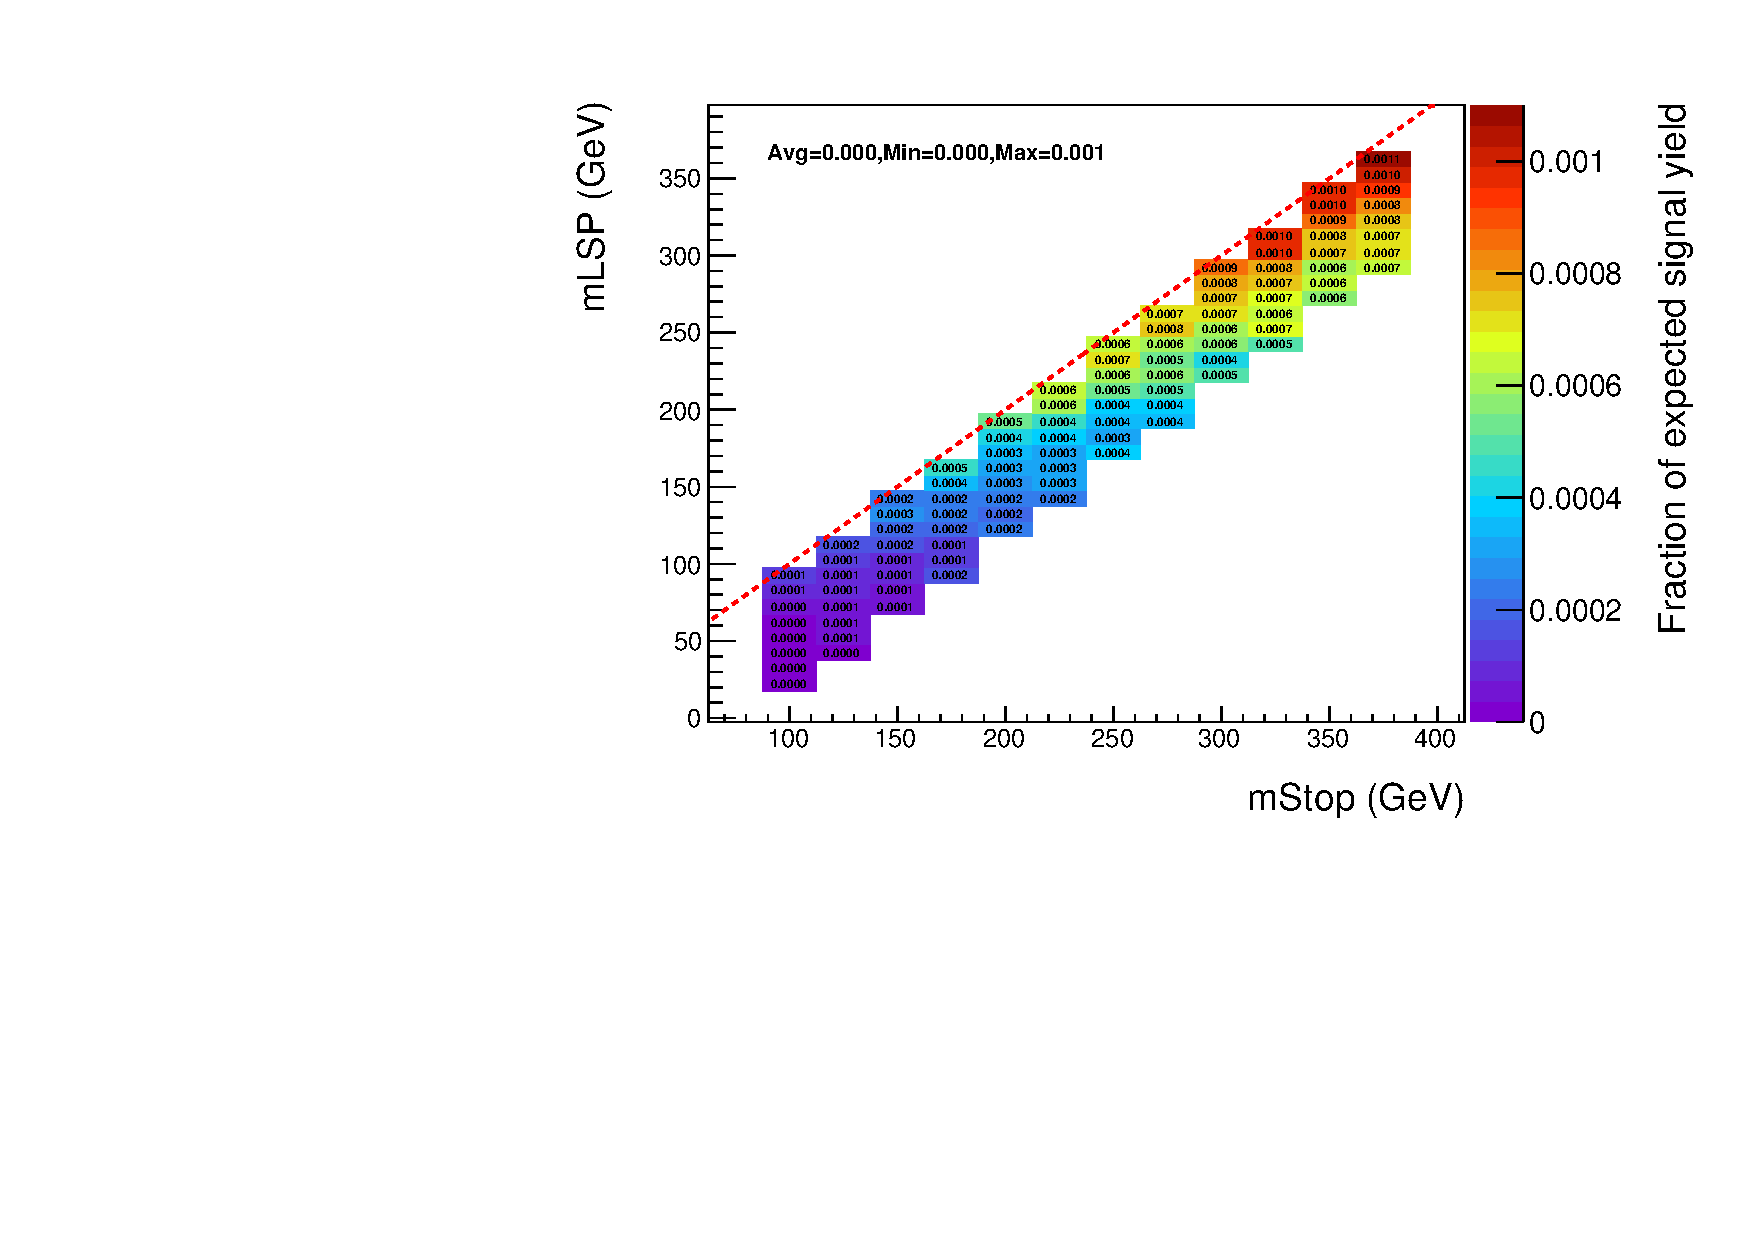
\includegraphics[width=0.4\textwidth]{figures/sms/t2_4body/v16/T2_4body_had_eff_maps_eq1b_le3j_SITV}
%    } 
%    \subfigure[\mj sample, (2--3,1)]{
%      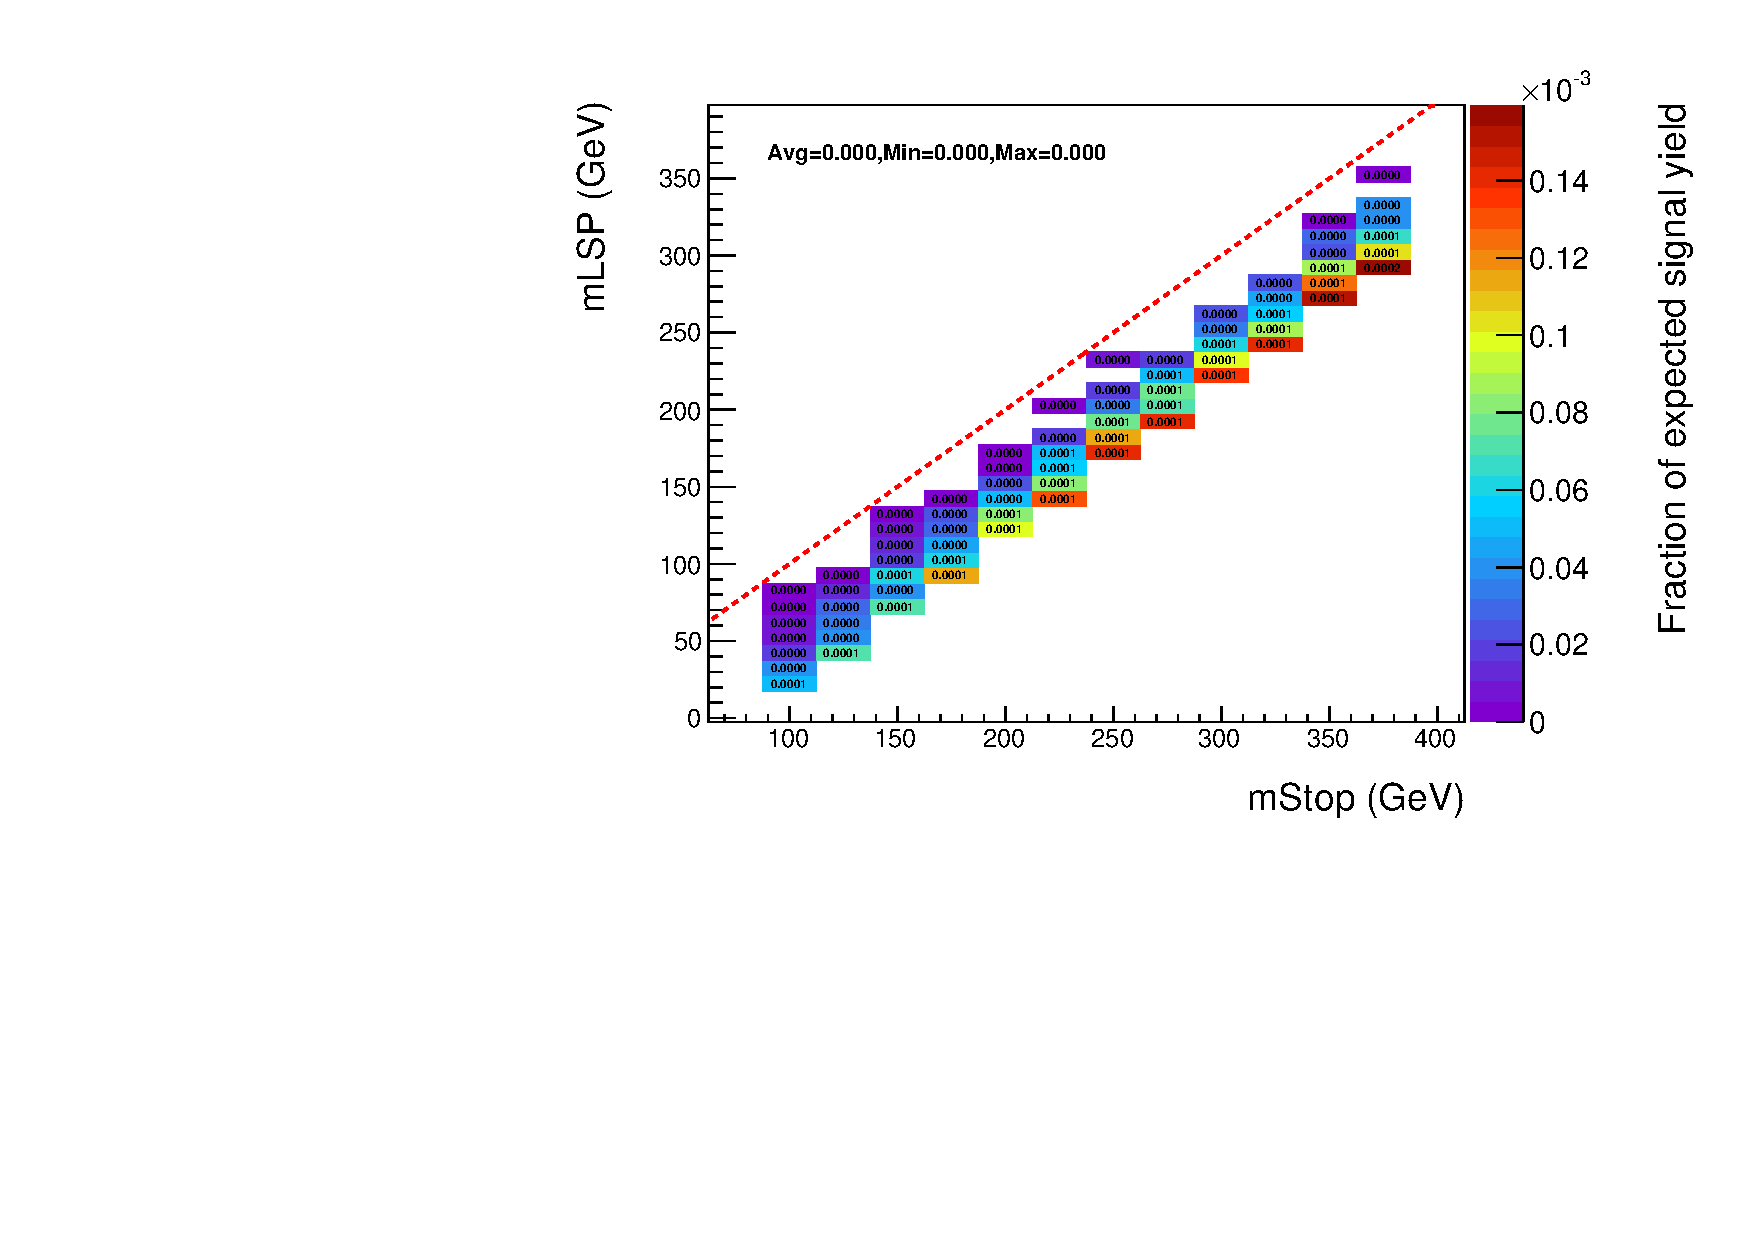
\includegraphics[width=0.4\textwidth]{figures/sms/t2_4body/v16/T2_4body_muon_eff_maps_eq1b_le3j_SITV}
%    } \\
%    \subfigure[Signal region, ($\geq 4$,0)]{
%      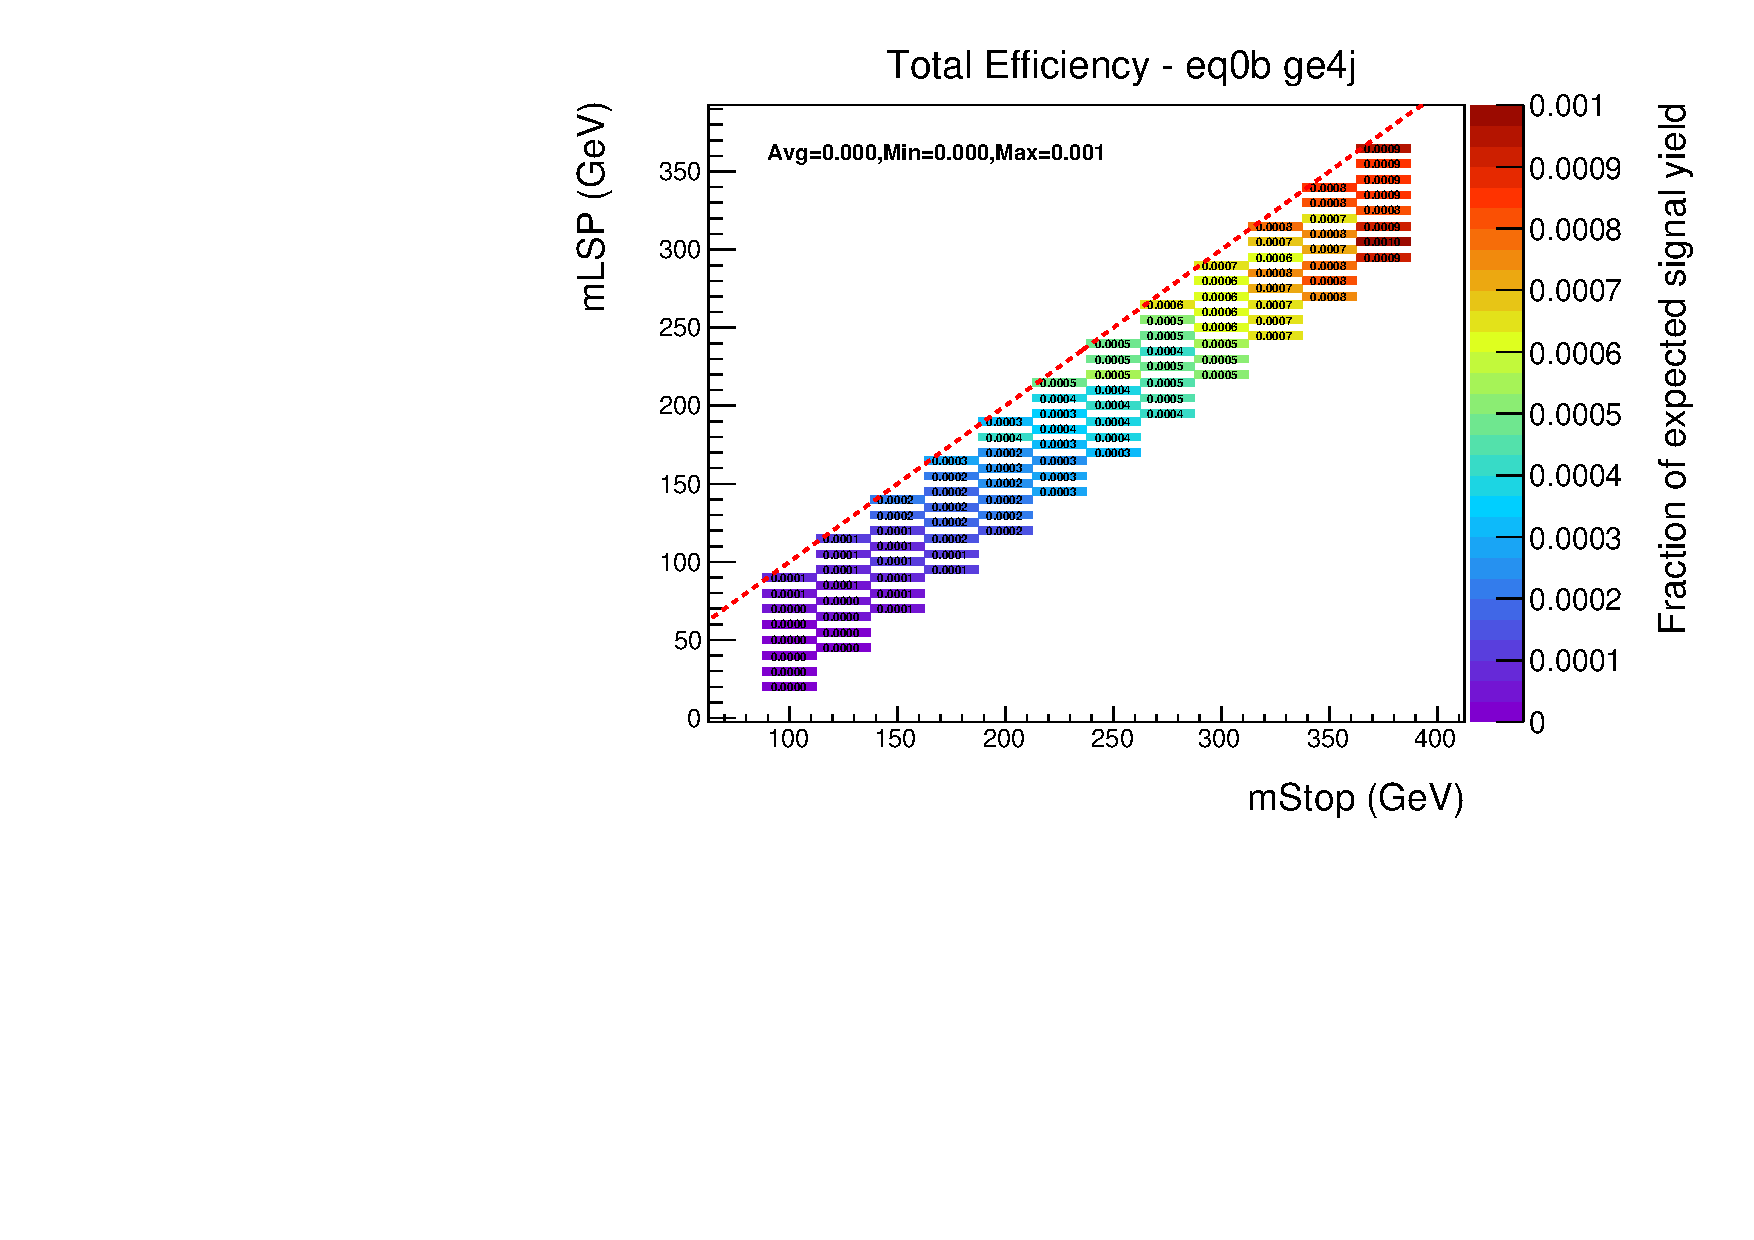
\includegraphics[width=0.4\textwidth]{figures/sms/t2_4body/v16/T2_4body_had_eff_maps_eq0b_ge4j_SITV}
%    } 
%    \subfigure[\mj sample, ($\geq 4$,0)]{
%      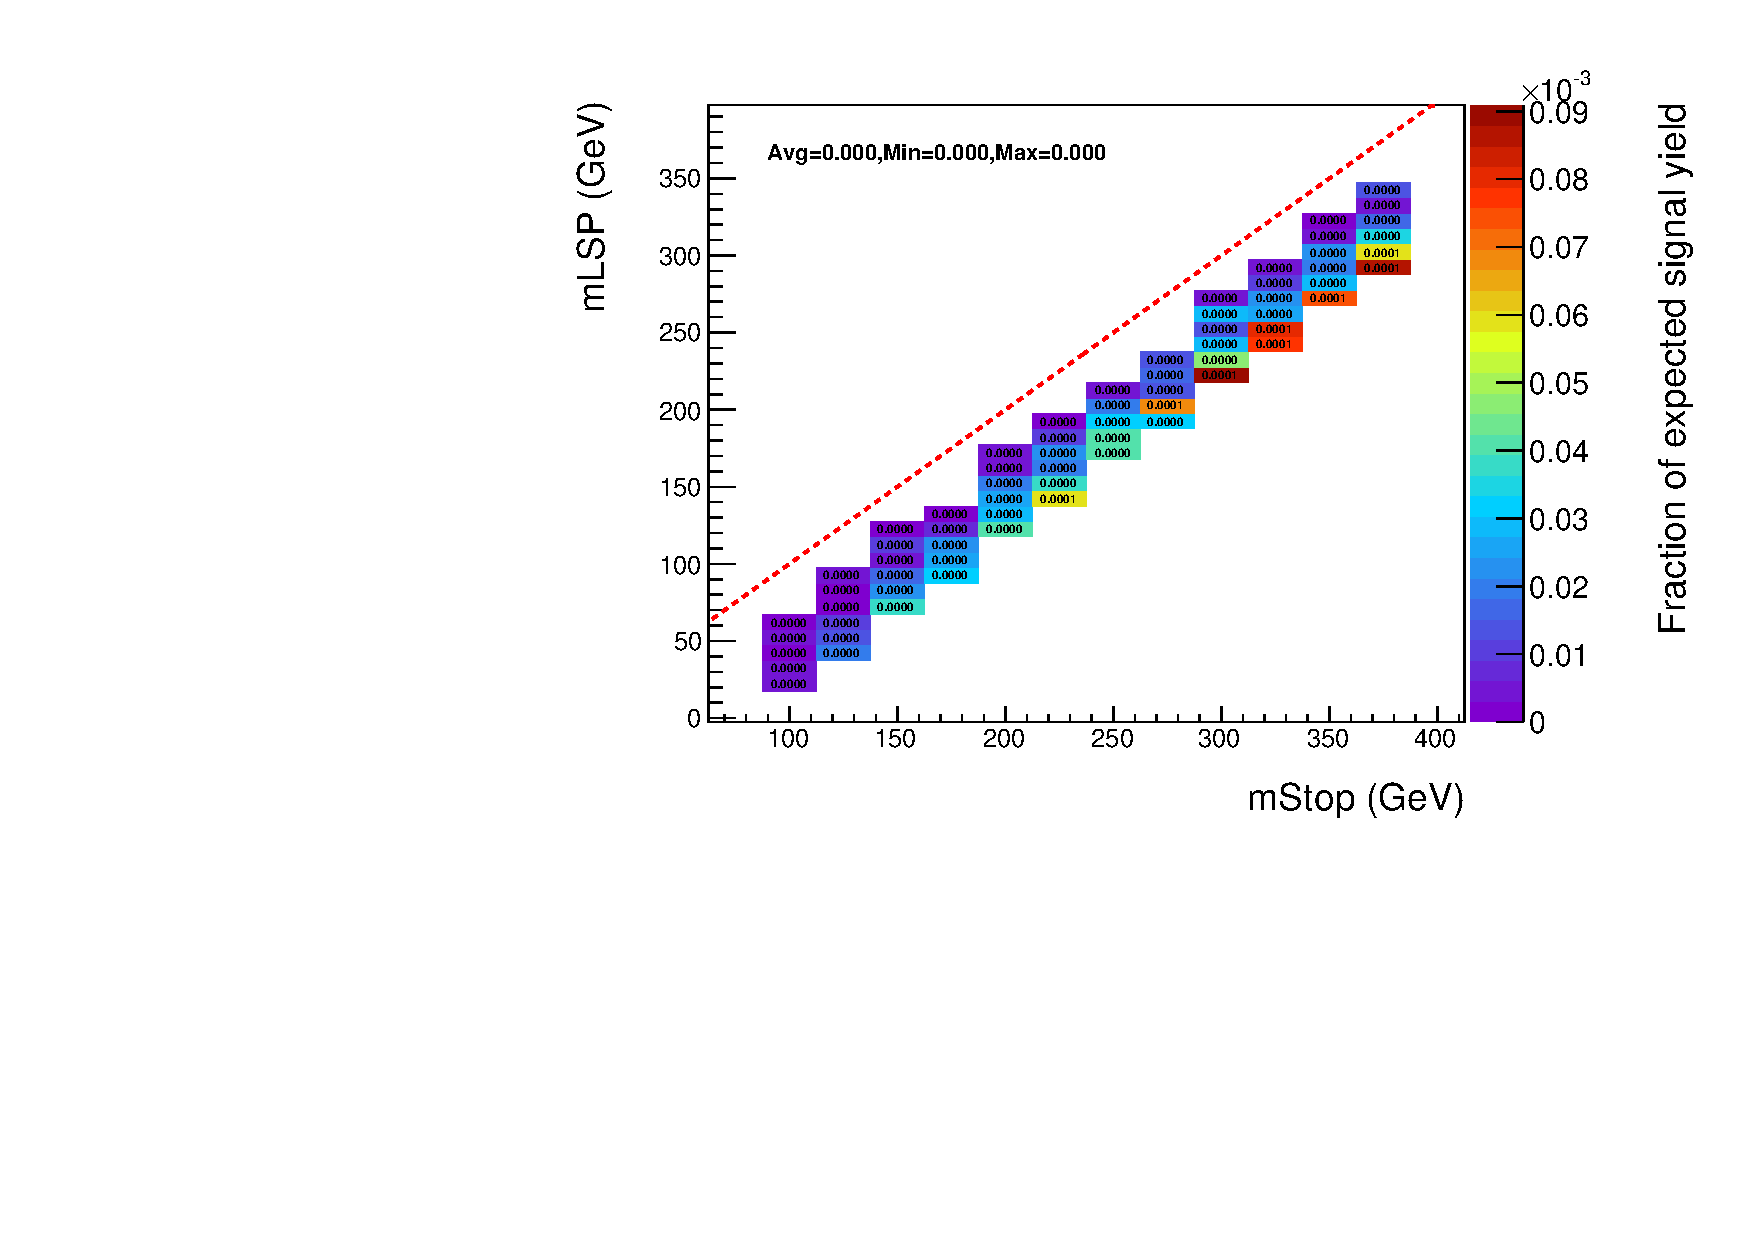
\includegraphics[width=0.4\textwidth]{figures/sms/t2_4body/v16/T2_4body_muon_eff_maps_eq0b_ge4j_SITV}
%    } \\
%    \subfigure[Signal region, ($\geq 4$,1)]{
%      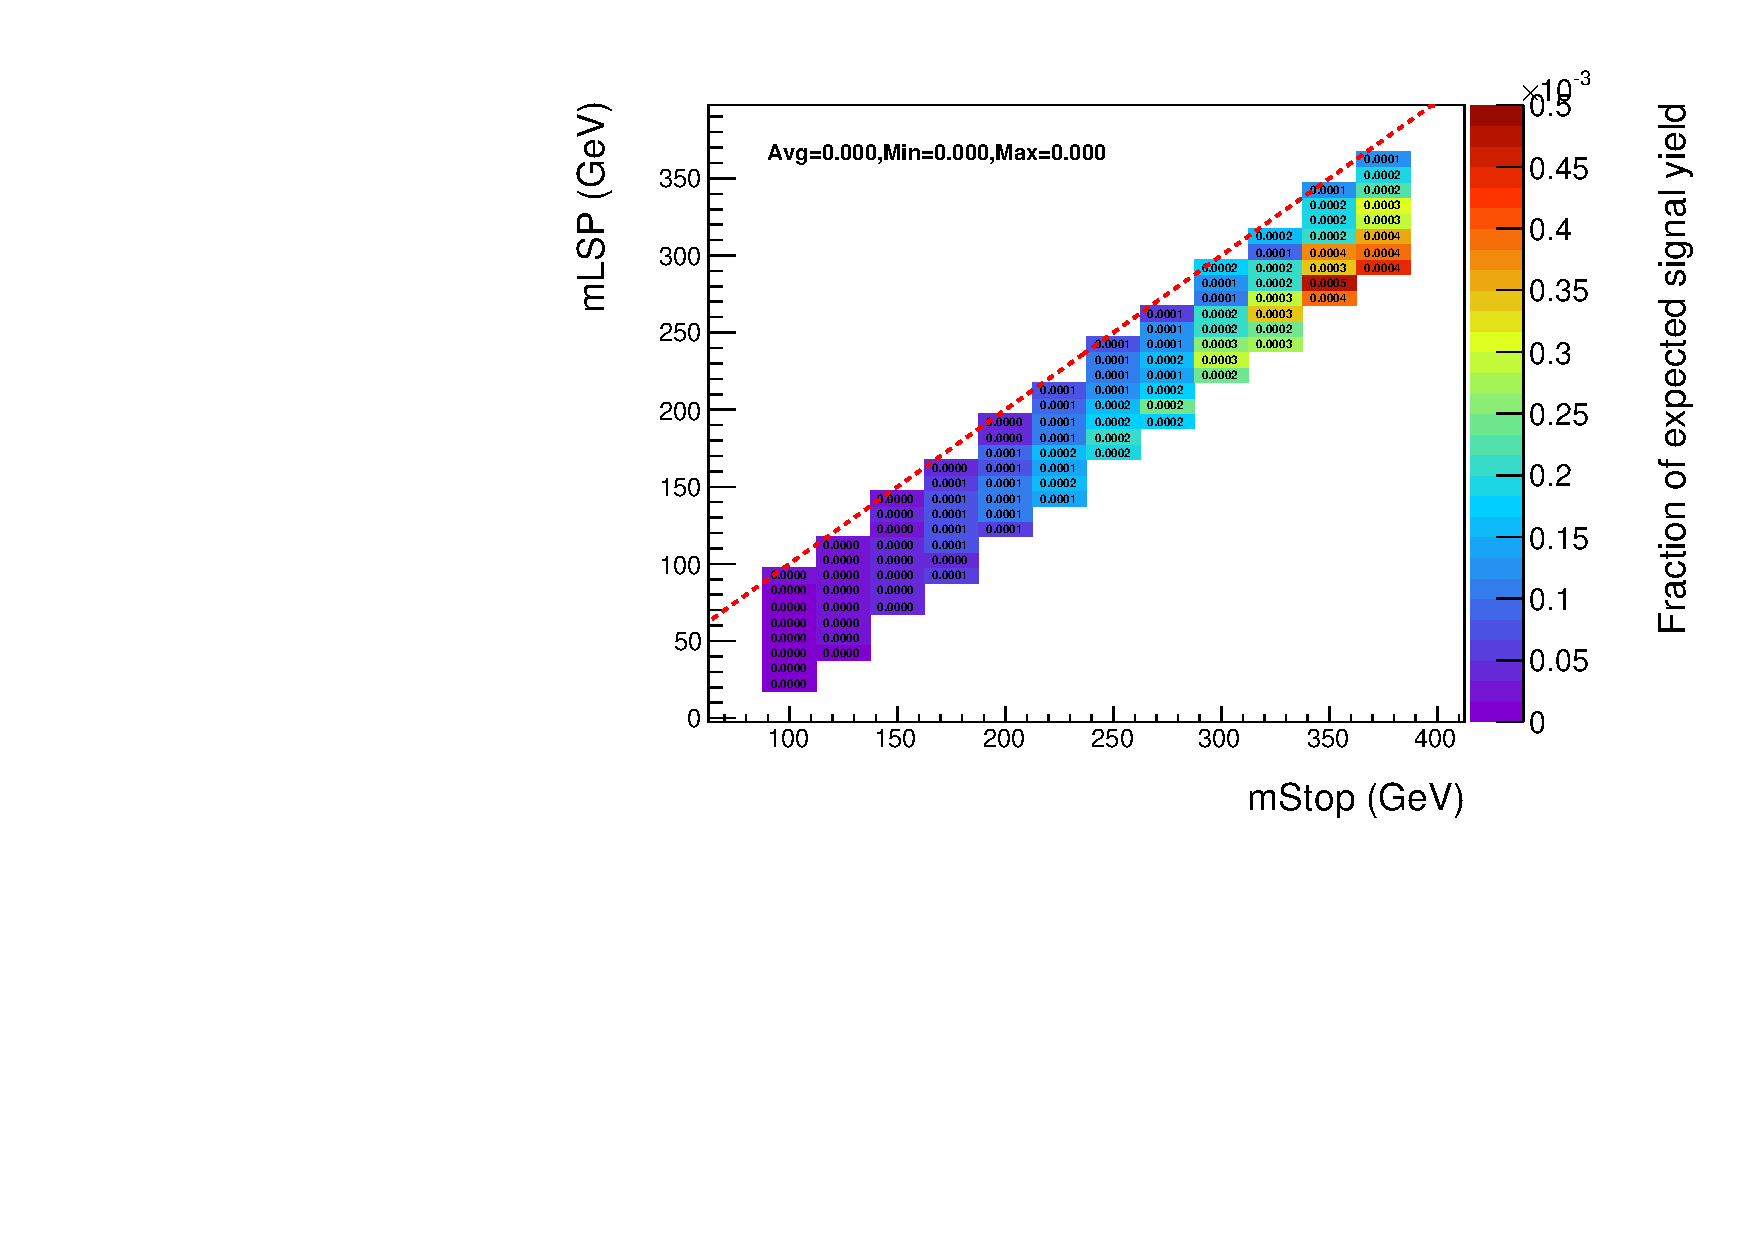
\includegraphics[width=0.4\textwidth]{figures/sms/t2_4body/v16/T2_4body_had_eff_maps_eq1b_ge4j_SITV}
%    } 
%    \subfigure[\mj sample, ($\geq 4$,1)]{
%      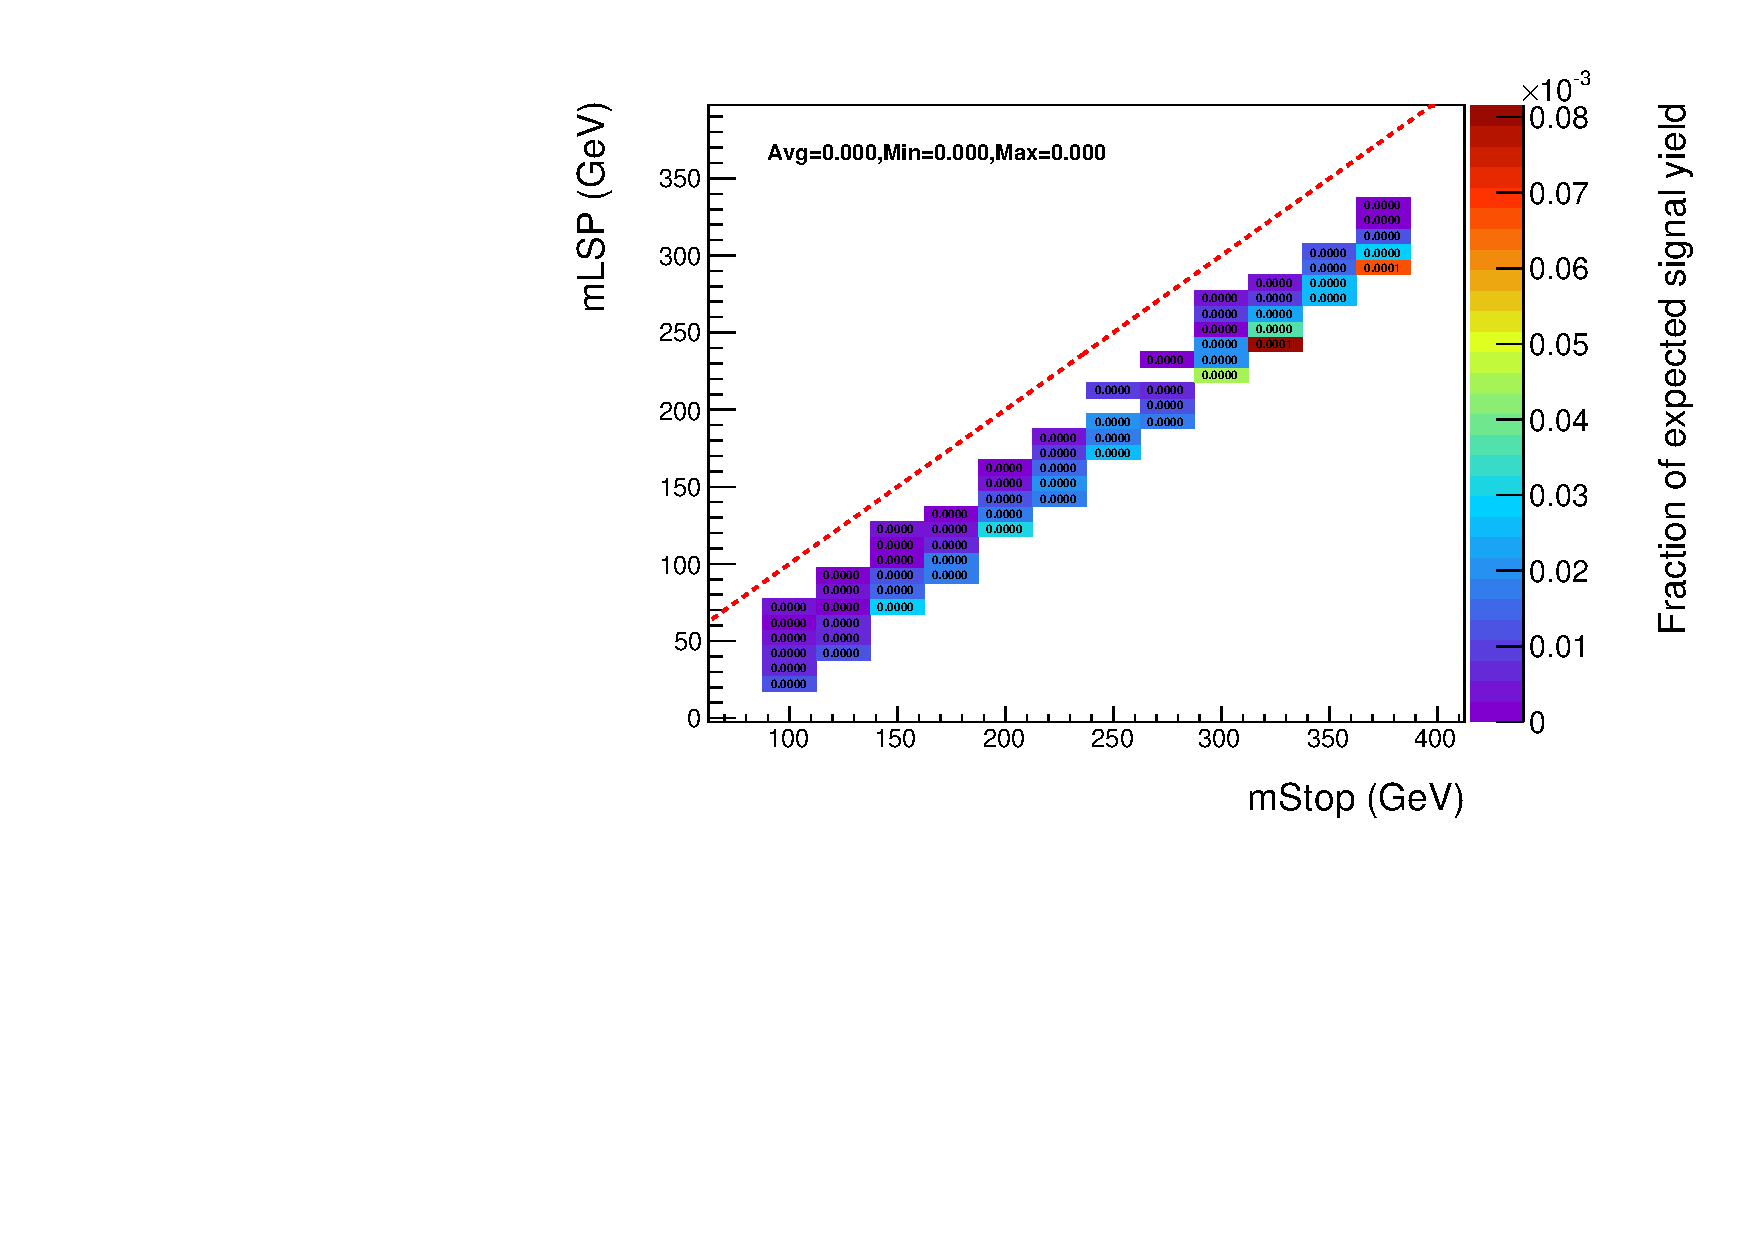
\includegraphics[width=0.4\textwidth]{figures/sms/t2_4body/v16/T2_4body_muon_eff_maps_eq1b_ge4j_SITV}
%    } \\
%    \caption{Signal efficiency times acceptance for the \texttt{T2\_4body}
%      in (left) the signal region and (right) the \mj control sample
%      (\ie, signal contamination) for the relevant event categories
%      defined by \njet and \nb. Note the different z-axis scales.}
%    \label{fig:sms-eff-t2_4body}
%  \end{center}
% \end{figure}

%********************************** % Second Section  *************************************
\section{Systematic Uncertainties on Signal Acceptance }  %Section - 1.2
\label{sec:interpretation_uncertainties}

Fully reliant on MC for signal interpretations.
A number of different considerations

\subsection{Jet energy scale}
\subsection{Initial State Radiation}
\subsection{Btag scale factors}
\subsection{PDF}
\subsection{MHT/MET cleaning cut}
\subsection{Dead ECAL Filter}
\subsection{Shape systematics}
\subsection{Integrated Luminosity}
\subsection{Number of MC Partons}
\subsection{Any others?}
\subsection{Summary}

%********************************** % Third Section  *************************************
\section{Limits on models of Supersymmetry}  %Section - 1.3
\label{sec:interpretation_limits}

\subsection{Overview of limit setting procedure}
Using green and blue band fits for expected and observed
considering MC stats of signal MC samples
point-by-point systematics

discussion of CLs method. Look up `CLs 4 LHC'

\subsection{Limits}
different limits for the various models


%********************************** % Fourth Section  *************************************
\section{Interpretation of excesses}
\label{sec:interpretation_excess}
best fit points in T2cc
global context?
p-values with SUSY assumption? is that even a thing? who knows? who cares.